% cd /storage/emulated/0/Documents/documents/latex/1920/Grade-10/2nd/inscribed-angles-and-intercepted-arcs && pdflatex hand-inscribed-angles-and-intercepted-arcs.tex && termux-open hand-inscribed-angles-and-intercepted-arcs.pdf


\documentclass[handout]{beamer} 

\usepackage{pgfpages} 
\mode<handout>{%
\pgfpagesuselayout{4 on 1}[
%letterpaper, 
legalpaper, %landscape, 
border shrink=1mm] 
%\setbeameroption{show notes} 
}

\usepackage{xcolor}
\usepackage{anyfontsize}
\usepackage{enumitem}
\usepackage{multicol}
\usepackage{amsmath}
%\usepackage{amsfonts,dsfont}% for \mathds 
\usepackage{tabularx, booktabs, makecell} 
\usepackage{gensymb}
\usepackage{multirow}
\usepackage{graphicx, tipa}
\usepackage{tikz}
\usetikzlibrary{angles,quotes}
\usepackage{pgfplots} 
\usetikzlibrary{calc}
\pgfplotsset{compat=newest}
\usetikzlibrary{arrows.meta}
\usetikzlibrary{intersections}
\usetikzlibrary{decorations.pathreplacing}
\usepackage{flafter}
\usepackage{amsmath,amssymb,cancel,units}
\usepackage{microtype} % nicer output 
\usepackage{hfoldsty} % nicer output 
\usepackage{fixltx2e} 
\usepackage{mathptmx}
%\usepackage{mnsymbol}
\usepackage{numprint}
\usepackage[utf8]{inputenc} 
\usepackage[T1]{fontenc}

\pagenumbering{gobble}
%\linespread{0.9}
\newcommand{\vspce}{\vspace{0.75ex}}
\newcommand{\hspce}{\hspace{0.5em}}

\newcommand{\vertadjust}{\vspace*{-2.5in}} % legalpaper
%\newcommand{\vertadjust}{\vspace*{-1.5in}} % letterpaper

\newcommand{\blank}{\underline{\hspace{2em}}}%{\rule{1em}{0.15ex}}
\newcommand{\arc}[1]{{% 
\setbox9=\hbox{#1}% 
\ooalign{\resizebox{\wd9}{\height}{\texttoptiebar{\phantom{A}}}\cr#1}}}

\newcolumntype{C}{ >{\centering\arraybackslash} X}

%\frame[shrink=5] 
\begin{document} 
\vertadjust
\begin{frame} %1
\begin{center}
\textbf{Inscribed Angles and Intercepted Arcs}
\end{center}

\vspace*{1ex}
\begin{center}
\scalebox{1}{
\noindent\begin{minipage}{\textwidth}
{
\textbf{Inscribed angle: } an angle whose vertex lies on the circle and whose sides are chords of a circle

\vspce 

The measure of an inscribed angle is \textbf{half} the measure of its intercepted arc.

\vspce 

In a circle, if two inscribed angles intercept the same arc or congruent arcs, then the angles are congruent.

\vspce 

An angle inscribed in a semicircle is a right angle and therefore the measure is equal to $90\degree$.

\vspce 

If a quadrilateral is inscribed in a circle, then its opposite angles are supplementary.
}
\end{minipage}}
\end{center} 

 
\def\currentdir{/storage/emulated/0/Documents/documents/latex/1920/Grade-10/2nd/inscribed-angles-and-intercepted-arcs}


\textbf{Practice Exercises}

\vspce

A. Refer to $ \odot O$ to answer the following. 
\begin{center}
\scalebox{1}{
\noindent\begin{minipage}{\textwidth}
{\begin{enumerate}[label = \arabic*. ]
\item Name the angle that  intercept \arc{AP}. 
\item Name the angles that  intercept \arc{EV}. 
\item Name the arc that is  intercepted by $\angle{PAE}$. 
\item Name the arc that is intercepted \\ by $\angle{EVP}$. \hspace*{6cm}\vspace*{1ex}\begin{tikzpicture}[dot/.style={circle, fill=black, inner sep=0pt, outer sep=0pt, minimum size=3pt}, 
dim-label/.style={fill=white, rectangle, inner sep=2pt, outer sep=0pt}, 
nodot/.style={circle, fill=black, inner sep=0pt, outer sep=0pt, minimum size=0pt}, 
remember picture, overlay
]  

\def\rad1{1.2cm}

% the origin 
\coordinate (o) at (0,0); 
% the circle and the dot at the origin
\draw[line width=0.5mm] (o) node[circle, fill=black, inner sep=0pt, outer sep=0pt, minimum size=3pt] {} circle [radius=\rad1]; 

\node(o-label) at ($(o)+(200:0.22*\rad1)$) {$O$};

\node (e) at (90:\rad1) [nodot] {}; 
\node(e-label) at ($(e)+(90:0.22*\rad1)$) {$E$};

\node (v) at (20:\rad1) [nodot] {}; 
\node(v-label) at ($(v)+(20:0.22*\rad1)$) {$V$};

\node (a) at (270:\rad1) [nodot] {}; 
\node(a-label) at ($(a)+(270:0.22*\rad1)$) {$A$};

\node (p) at (180:\rad1) [nodot] {}; 
\node(p-label) at ($(p)+(180:0.22*\rad1)$) {$P$};

\node(r-label) at ($(o)+(115:0.4*\rad1)$) {$R$};

\draw[line width=0.3mm] (a)--(e); 
\draw[line width=0.3mm] (p)--(v); 
\draw[line width=0.3mm] (p)--(e)--(v) --(a) --(p) ; 

\node (Name) at (-45:1.3*\rad1) {$\odot{O}$}; 
\end{tikzpicture}

 
%\vspace*{-3ex}
\item If $m\angle{PEA}=48\degree $, then $m\arc{AP}=\blank$ \\ and $m\angle{AVP}=\blank$. 
\item $m\angle{EPA}=\blank$
\item $m\angle{EVP}+m\angle{PVA}=\blank$
\item  If $m\angle{VEP}=100\degree $, then $m\angle{PAV}=\blank$.
\end{enumerate}
}
\end{minipage}}
\end{center} 
%\begin{tikzpicture}[dot/.style={circle, fill=black, inner sep=0pt, outer sep=0pt, minimum size=3pt}, 
dim-label/.style={fill=white, rectangle, inner sep=2pt, outer sep=0pt}, 
nodot/.style={circle, fill=black, inner sep=0pt, outer sep=0pt, minimum size=0pt}, 
remember picture, overlay
]  

\def\rad1{1.2cm}

% the origin 
\coordinate (o) at (0,0); 
% the circle and the dot at the origin
\draw[line width=0.5mm] (o) node[circle, fill=black, inner sep=0pt, outer sep=0pt, minimum size=3pt] {} circle [radius=\rad1]; 

\node(o-label) at ($(o)+(200:0.22*\rad1)$) {$O$};

\node (e) at (90:\rad1) [nodot] {}; 
\node(e-label) at ($(e)+(90:0.22*\rad1)$) {$E$};

\node (v) at (20:\rad1) [nodot] {}; 
\node(v-label) at ($(v)+(20:0.22*\rad1)$) {$V$};

\node (a) at (270:\rad1) [nodot] {}; 
\node(a-label) at ($(a)+(270:0.22*\rad1)$) {$A$};

\node (p) at (180:\rad1) [nodot] {}; 
\node(p-label) at ($(p)+(180:0.22*\rad1)$) {$P$};

\node(r-label) at ($(o)+(115:0.4*\rad1)$) {$R$};

\draw[line width=0.3mm] (a)--(e); 
\draw[line width=0.3mm] (p)--(v); 
\draw[line width=0.3mm] (p)--(e)--(v) --(a) --(p) ; 

\node (Name) at (-45:1.3*\rad1) {$\odot{O}$}; 
\end{tikzpicture}




\def\currentdir{/storage/emulated/0/Documents/documents/latex/1920/Grade-10/2nd/inscribed-angles-and-intercepted-arcs}

\begin{center}
\scalebox{1}{
\noindent\begin{minipage}{\textwidth}
{
B. Given $\odot{S}, \overline{AR}\cong\overline{RO}\cong \overline{OS}\cong\overline{SA}, m\angle{AMR}=3x+20$ and $m\angle{OMR}=x+30$. Find each measure. 
\begin{enumerate}[label = \arabic*. ]
\item $x$
\item $m\angle{AMR}$
\item $m\angle{ORM}$
\item $m\arc{AM}$
\item $m\angle{RNO}$ \hspace*{4cm}
\begin{tikzpicture}[dot/.style={circle, fill=black, inner sep=0pt, outer sep=0pt, minimum size=3pt}, 
dim-label/.style={fill=white, rectangle, inner sep=2pt, outer sep=0pt}, 
nodot/.style={circle, fill=black, inner sep=0pt, outer sep=0pt, minimum size=0pt}, 
remember picture, overlay
]  

\def\rad3{1.5cm}

\coordinate (s) at (0,0);

\node (s-label) at ($(s)+ (-40:0.22*\rad3)$) {$S$}; 

\node (n-label) at ($(s)+ (80:0.65*\rad3)$) {$N$};

\draw[line width=0.5mm] (s) node[circle, fill=black, inner sep=0pt, outer sep=0pt, minimum size=3pt] {} circle [radius=\rad3]; 

\node (o) at (30:\rad3) [nodot] {};

\node (o-label) at ($(o)+ (30:0.22*\rad3  )$) {$O$};

\node (r) at (90:\rad3) [nodot] {}; 

\node (r-label) at ($(r)+ (90:0.22*\rad3  )$) {$R$};

\node (a) at (150:\rad3) [nodot] {};

\node (a-label) at ($(a)+ (150:0.22*\rad3 )$) {$A$};

\node (m) at (270:\rad3) [nodot] {};

\node (m-label) at ($(m)+ (270:0.22*\rad3  )$) {$ \  M$}; 

\draw[line width=0.3mm] (r)--(m)--(o)--(r)--(a)--(s)--(o)--(m)--(a)--(o) ; 
 
 
\node(name) at ($(s)+ (310:1.3*\rad3)$) {$\odot{S}$};
 
\end{tikzpicture} 
\item $m\angle{RAM}$
\item $m\arc{AR}$
\item $m\arc{OM}$
\item $m\angle{ROM}$
\item $m\angle{AMO}$
\end{enumerate}
}
\end{minipage}}
\end{center} 
%
\begin{tikzpicture}[dot/.style={circle, fill=black, inner sep=0pt, outer sep=0pt, minimum size=3pt}, 
dim-label/.style={fill=white, rectangle, inner sep=2pt, outer sep=0pt}, 
nodot/.style={circle, fill=black, inner sep=0pt, outer sep=0pt, minimum size=0pt}, 
remember picture, overlay
]  

\def\rad3{1.5cm}

\coordinate (s) at (0,0);

\node (s-label) at ($(s)+ (-40:0.22*\rad3)$) {$S$}; 

\node (n-label) at ($(s)+ (80:0.65*\rad3)$) {$N$};

\draw[line width=0.5mm] (s) node[circle, fill=black, inner sep=0pt, outer sep=0pt, minimum size=3pt] {} circle [radius=\rad3]; 

\node (o) at (30:\rad3) [nodot] {};

\node (o-label) at ($(o)+ (30:0.22*\rad3  )$) {$O$};

\node (r) at (90:\rad3) [nodot] {}; 

\node (r-label) at ($(r)+ (90:0.22*\rad3  )$) {$R$};

\node (a) at (150:\rad3) [nodot] {};

\node (a-label) at ($(a)+ (150:0.22*\rad3 )$) {$A$};

\node (m) at (270:\rad3) [nodot] {};

\node (m-label) at ($(m)+ (270:0.22*\rad3  )$) {$ \  M$}; 

\draw[line width=0.3mm] (r)--(m)--(o)--(r)--(a)--(s)--(o)--(m)--(a)--(o) ; 
 
 
\node(name) at ($(s)+ (310:1.3*\rad3)$) {$\odot{S}$};
 
\end{tikzpicture} 
%\def\currentdir{/storage/emulated/0/Documents/documents/latex/1920/Grade-10/2nd/inscribed-angles-and-intercepted-arcs}

\textbf{Problem Set}

\vspce

A. Use the
given figures to find the value of $x$ and $y$. 
\begin{center}
\scalebox{1}{
\noindent\begin{minipage}{\textwidth}
{\begin{enumerate}[label = \arabic*. ]
\begin{multicols}{2}
%1
\item \hspce \def\rad2{1.2cm}
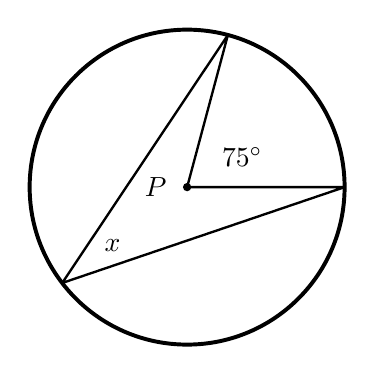
\begin{tikzpicture}[dot/.style={circle, fill=black, inner sep=0pt, outer sep=0pt, minimum size=3pt}, 
dim-label/.style={fill=white, rectangle, inner sep=2pt, outer sep=0pt}, 
nodot/.style={circle, fill=black, inner sep=0pt, outer sep=0pt, minimum size=0pt}, 
%remember picture, overlay
baseline = (current bounding box.west)
]  

% the origin 
\coordinate (p) at (0,0); 
% the circle and the nodot at the origin
\draw[line width=0.5mm] (p) node[circle, fill=black, inner sep=0pt, outer sep=0pt, minimum size=3pt] {} circle [radius=\rad2]; 

\node(p-label) at ($(p)+(180:0.2*\rad2)$) {$P$};

\node(p-angle) at ($(p)+(29:0.4*\rad2)$) {$75\degree$};

\node (a) at (0:\rad2) [nodot] {}; 

\node (b) at (75:\rad2) [nodot] {}; 


\node (c) at (217.5:\rad2) [nodot] {}; 

\node(x-label) at ($(c)+(37:0.4*\rad2)$) {$x$};


\draw[line width=0.3mm] (p)--(a)--(c) --(b) --(p) ; 


\end{tikzpicture} 
%2
\item \hspce 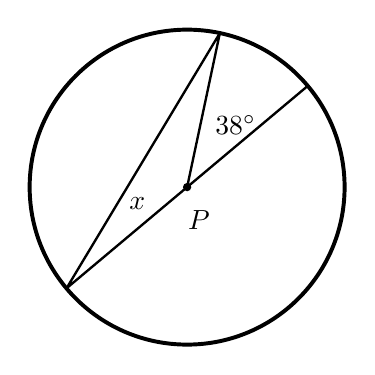
\begin{tikzpicture}[dot/.style={circle, fill=black, inner sep=0pt, outer sep=0pt, minimum size=3pt}, 
dim-label/.style={fill=white, rectangle, inner sep=2pt, outer sep=0pt}, 
nodot/.style={circle, fill=black, inner sep=0pt, outer sep=0pt, minimum size=0pt}, 
%remember picture, overlay
baseline = (current bounding box.west)
]  

\coordinate (p) at (0,0); 

\draw[line width=0.5mm] (p) node[circle, fill=black, inner sep=0pt, outer sep=0pt, minimum size=3pt] {} circle [radius=\rad2]; 

\node(p-label) at ($(p)+(290:0.22*\rad2)$) {$P$};

\node(p-angle) at ($(p)+(52:0.5*\rad2)$) {${38\degree}$};

\node (a) at (40:\rad2) [nodot] {}; 

\node (b) at (78:\rad2) [nodot] {}; 

\node (c) at (220:\rad2) [nodot] {};

\node(x-label) at ($(c)+(50:0.7*\rad2)$) {${x}$};
 
\draw[line width=0.3mm] (a)--(c)--(b)--(p) ; 

\end{tikzpicture} 
%3
\item \hspce 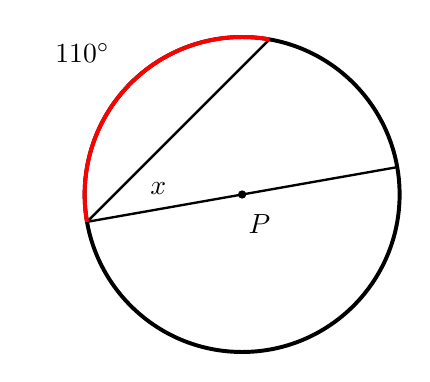
\begin{tikzpicture}[dot/.style={circle, fill=black, inner sep=0pt, outer sep=0pt, minimum size=3pt}, 
dim-label/.style={fill=white, rectangle, inner sep=2pt, outer sep=0pt}, 
nodot/.style={circle, fill=black, inner sep=0pt, outer sep=0pt, minimum size=0pt}, 
%remember picture, overlay
baseline = (current bounding box.west)
]  
\coordinate (p) at (0,0); 

\draw[line width=0.5mm] (p) node[circle, fill=black, inner sep=0pt, outer sep=0pt, minimum size=3pt] {} circle [radius=\rad2]; 

\node(p-label) at ($(p)+(-60:0.22*\rad2)$) {${P}$};

\node(angle) at ($(p)+(140:1.4*\rad2)$) {$ \  \ {110\degree}$};

\node (a) at (10:\rad2) [nodot] {}; 

\node (b) at (80:\rad2) [nodot] {}; 

\node (c) at (190:\rad2) [nodot] {};

\node(x-label) at ($(c)+(25:0.5*\rad2)$) {${x}$};
 
\draw[line width=0.3mm] (a)--(c) --(b); 

\draw[red, line width=0.5mm] (b)  arc (80:190:\rad2);

\end{tikzpicture} 
%4
\item \hspce 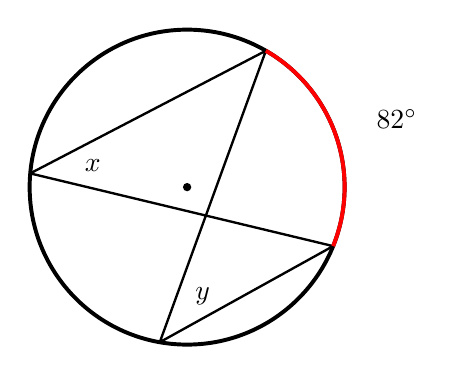
\begin{tikzpicture}[dot/.style={circle, fill=black, inner sep=0pt, outer sep=0pt, minimum size=3pt}, 
dim-label/.style={fill=white, rectangle, inner sep=2pt, outer sep=0pt}, 
nodot/.style={circle, fill=black, inner sep=0pt, outer sep=0pt, minimum size=0pt}, 
%remember picture, overlay
baseline = (current bounding box.west)
]  

\coordinate (p) at (0,0); 

\draw[line width=0.5mm] (p) node[circle, fill=black, inner sep=0pt, outer sep=0pt, minimum size=3pt] {} circle [radius=\rad2];
 
%\node(p-label) at ($(p)+(180:15pt)$) {$ \  \ {P}$};
\node(angle) at ($(p)+(18:1.4*\rad2)$) {${82\degree}$};

\node (a) at (60:\rad2) [nodot] {}; 

\node (b) at (175:\rad2) [nodot] {}; 

\node (c) at (260:\rad2) [nodot] {}; 

\node (d) at (-22:\rad2) [nodot] {};

\node(x-label) at ($(b)+(7:0.4*\rad2)$) {${x}$};

\node(y-label) at ($(c)+(47:0.4*\rad2)$) {${y}$};
 
\draw[line width=0.3mm] (a)--(b) --(d) --(c)--(a); 

\draw[red, line width=0.5mm] (d)  arc (-22:60:\rad2);

\end{tikzpicture} 
%5
\item \hspce 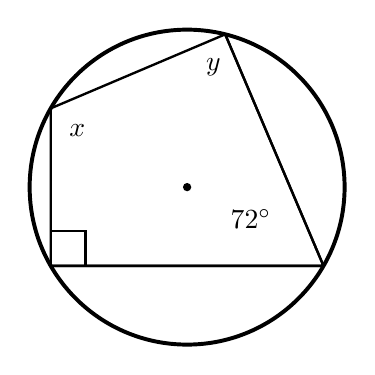
\begin{tikzpicture}[dot/.style={circle, fill=black, inner sep=0pt, outer sep=0pt, minimum size=3pt}, 
dim-label/.style={fill=white, rectangle, inner sep=2pt, outer sep=0pt}, 
nodot/.style={circle, fill=black, inner sep=0pt, outer sep=0pt, minimum size=0pt}, 
%remember picture, overlay
baseline = (current bounding box.west)
]  

\coordinate (p) at (0,0); 

\draw[line width=0.5mm] (p) node[circle, fill=black, inner sep=0pt, outer sep=0pt, minimum size=3pt] {} circle [radius=\rad2]; 

\node (a) at (76:\rad2) [nodot] {};

\node(y-label) at ($(a)+(250:0.22*\rad2)$) {${y}$};
  
\node (b) at (150:\rad2) [nodot] {};

\node(x-label) at ($(b)+(-40:0.22*\rad2)$) {${x}$};
 
\node (c) at (210:\rad2) [nodot] {}; 

\draw[line width=0.3mm] (c) rectangle ++(0.22*\rad2,0.22*\rad2) node[]{};

\node (d) at (-30:\rad2) [nodot] {}; 

\draw [line width=0.3mm](a) -- (d) -- (c) pic [draw,angle radius=0.3*\rad2] {angle = a--d--c}; 

\node(d-angle) at ($(d)+(150:0.6*\rad2)$) {$ \  \ {72\degree}$};

\draw[line width=0.3mm] (a)--(b) --(c) --(d) --(a) ; 

\end{tikzpicture} 
%6
\item \hspce 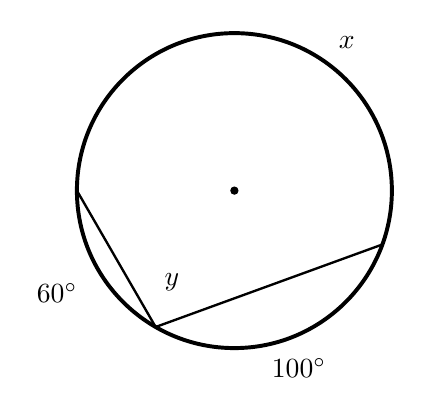
\begin{tikzpicture}[dot/.style={circle, fill=black, inner sep=0pt, outer sep=0pt, minimum size=3pt}, 
dim-label/.style={fill=white, rectangle, inner sep=2pt, outer sep=0pt}, 
nodot/.style={circle, fill=black, inner sep=0pt, outer sep=0pt, minimum size=0pt}, 
%remember picture, overlay
baseline = (current bounding box.west)
]  

\coordinate (p) at (0,0); 

\draw[line width=0.5mm] (p) node[circle, fill=black, inner sep=0pt, outer sep=0pt, minimum size=3pt] {} circle [radius=\rad2]; 

\node (a) at (180:\rad2) [nodot] {}; 

\node (b) at (240:\rad2) [nodot] {};

\node(y-label) at ($(b)+(70:0.3*\rad2)$) {${y}$};
 
\node (c) at (340:\rad2) [nodot] {}; 

\node(ab) at ($(p)+(210:1.3*\rad2)$) {${60\degree}$};

\node(x-label) at ($(c)+(100:1.3*\rad2)$) {$x$};
 
\node(bc) at ($(p)+(290:1.2*\rad2)$) {${100\degree}$};

\draw[line width=0.3mm] (a)--(b) --(c); 

\end{tikzpicture} 
%7
\item \hspce 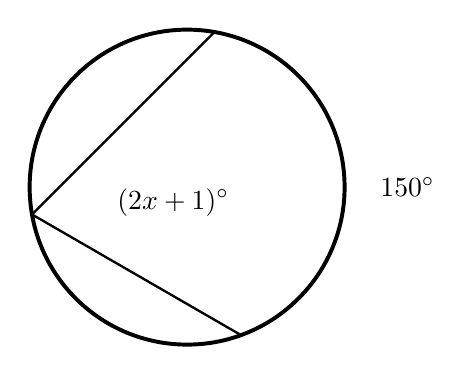
\begin{tikzpicture}[dot/.style={circle, fill=black, inner sep=0pt, outer sep=0pt, minimum size=3pt}, 
dim-label/.style={fill=white, rectangle, inner sep=2pt, outer sep=0pt}, 
nodot/.style={circle, fill=black, inner sep=0pt, outer sep=0pt, minimum size=0pt}, 
%remember picture, overlay
baseline = (current bounding box.west)
]  

\coordinate (p) at (0,0); 

\draw[line width=0.5mm] (p) node[circle, fill=black, inner sep=0pt, outer sep=0pt, minimum size=0pt] {} circle [radius=\rad2]; 

\node (a) at (80:\rad2) [nodot] {}; 

\node (b) at (190:\rad2) [nodot] {}; 

\node (c) at (-70:\rad2) [nodot] {}; 

\draw[line width=0.3mm] (a)--(b)--(c); 

\node(measure) at ($(b)+(5:0.9*\rad2)$) {${(2x+1)\degree}$};
 
\node(angle) at ($(p)+(0:1.4*\rad2)$) {${150\degree}$};
 
\end{tikzpicture} 
%8
\item \hspce 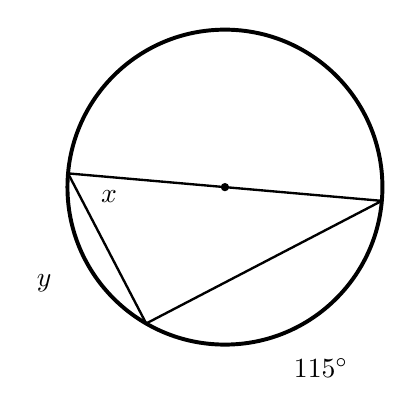
\begin{tikzpicture}[dot/.style={circle, fill=black, inner sep=0pt, outer sep=0pt, minimum size=3pt}, 
dim-label/.style={fill=white, rectangle, inner sep=2pt, outer sep=0pt}, 
nodot/.style={circle, fill=black, inner sep=0pt, outer sep=0pt, minimum size=0pt}, 
%remember picture, overlay
baseline = (current bounding box.west)
]  

\coordinate (p) at (0,0); 

\draw[line width=0.5mm] (p) node[circle, fill=black, inner sep=0pt, outer sep=0pt, minimum size=3pt] {} circle [radius=\rad2]; 

\node (a) at (-5:\rad2) [nodot] {}; 

\node (b) at (175:\rad2) [nodot] {}; 

\node (c) at (240:\rad2) [nodot] {}; 

\draw[line width=0.3mm] (a)--(b)--(c)--(a) ; 
 
\node(y-label) at ($(p)+(208:1.3*\rad2)$) {${y}$};
 
\node(x-label) at ($(b)+(-30:0.3*\rad2)$) {${x}$};
 
\node(115) at ($(p)+(298:1.3*\rad2)$) {${115\degree}$};
 
\end{tikzpicture} 
\end{multicols}
\end{enumerate}}     
\end{minipage}}
\end{center} 

B. $\Delta$GOA is inscribed in $\odot L$. If $m\angle{OGA}=75\degree$ and $m\arc{AG}=160\degree$, find: 
\begin{center}
\scalebox{1}{
\noindent\begin{minipage}{\textwidth}
 
{\begin{enumerate}[label = \arabic*. ]
\item $m\arc{OA}$ 
\item $m\arc{OG}$
\item $m\angle{GOA}$ \hspace*{3cm}\begin{tikzpicture}[dot/.style={circle, fill=black, inner sep=0pt, outer sep=0pt, minimum size=3pt}, 
dim-label/.style={fill=white, rectangle, inner sep=2pt, outer sep=0pt}, 
nodot/.style={circle, fill=black, inner sep=0pt, outer sep=0pt, minimum size=0pt}, 
remember picture, overlay
]  

\def\rad4{1.3cm}

\coordinate (l) at (0,0); 

\node(l-label) at ($(l)+(30:0.22*\rad4)$) {$L$};

\draw[line width=0.5mm] (l) node[circle, fill=black, inner sep=0pt, outer sep=0pt, minimum size=3pt] {} circle [radius=\rad4]; 

\node (a) at (15:\rad4) [nodot] {}; 

\node(a-label) at ($(a)+(15:0.22*\rad4)$) {$A$};
  
\node (o) at (165:\rad4) [nodot] {}; 

\node(o-label) at ($(o)+(165:0.22*\rad4)$) {$O$};
  
\node (g) at (215:\rad4) [nodot] {};

\node(g-label) at ($(g)+(215:0.22*\rad4)$) {$G$};
   
\node(75) at ($(g)+(53:0.4*\rad4)$) {$75\degree$};

\draw[line width=0.3mm] (a)--(o)--(g)--(a) ; 
 
\node(160) at ($(l)+(-45:1.3*\rad4)$) {$160\degree$};

\draw[red, line width=0.5mm] (a)  arc (15:-145:\rad4);

\end{tikzpicture} 
\item $m\angle{GAO}$  
\end{enumerate}}
\end{minipage}}
\end{center} 
\end{frame}

\vertadjust
\begin{frame} %2
%\begin{center}
\textbf{Inscribed Angles and Intercepted Arcs}
\end{center}

\vspace*{1ex}
\begin{center}
\scalebox{1}{
\noindent\begin{minipage}{\textwidth}
{
\textbf{Inscribed angle: } an angle whose vertex lies on the circle and whose sides are chords of a circle

\vspce 

The measure of an inscribed angle is \textbf{half} the measure of its intercepted arc.

\vspce 

In a circle, if two inscribed angles intercept the same arc or congruent arcs, then the angles are congruent.

\vspce 

An angle inscribed in a semicircle is a right angle and therefore the measure is equal to $90\degree$.

\vspce 

If a quadrilateral is inscribed in a circle, then its opposite angles are supplementary.
}
\end{minipage}}
\end{center} 

 
%\def\currentdir{/storage/emulated/0/Documents/documents/latex/1920/Grade-10/2nd/inscribed-angles-and-intercepted-arcs}


\textbf{Practice Exercises}

\vspce

A. Refer to $ \odot O$ to answer the following. 
\begin{center}
\scalebox{1}{
\noindent\begin{minipage}{\textwidth}
{\begin{enumerate}[label = \arabic*. ]
\item Name the angle that  intercept \arc{AP}. 
\item Name the angles that  intercept \arc{EV}. 
\item Name the arc that is  intercepted by $\angle{PAE}$. 
\item Name the arc that is intercepted \\ by $\angle{EVP}$. \hspace*{6cm}\vspace*{1ex}\begin{tikzpicture}[dot/.style={circle, fill=black, inner sep=0pt, outer sep=0pt, minimum size=3pt}, 
dim-label/.style={fill=white, rectangle, inner sep=2pt, outer sep=0pt}, 
nodot/.style={circle, fill=black, inner sep=0pt, outer sep=0pt, minimum size=0pt}, 
remember picture, overlay
]  

\def\rad1{1.2cm}

% the origin 
\coordinate (o) at (0,0); 
% the circle and the dot at the origin
\draw[line width=0.5mm] (o) node[circle, fill=black, inner sep=0pt, outer sep=0pt, minimum size=3pt] {} circle [radius=\rad1]; 

\node(o-label) at ($(o)+(200:0.22*\rad1)$) {$O$};

\node (e) at (90:\rad1) [nodot] {}; 
\node(e-label) at ($(e)+(90:0.22*\rad1)$) {$E$};

\node (v) at (20:\rad1) [nodot] {}; 
\node(v-label) at ($(v)+(20:0.22*\rad1)$) {$V$};

\node (a) at (270:\rad1) [nodot] {}; 
\node(a-label) at ($(a)+(270:0.22*\rad1)$) {$A$};

\node (p) at (180:\rad1) [nodot] {}; 
\node(p-label) at ($(p)+(180:0.22*\rad1)$) {$P$};

\node(r-label) at ($(o)+(115:0.4*\rad1)$) {$R$};

\draw[line width=0.3mm] (a)--(e); 
\draw[line width=0.3mm] (p)--(v); 
\draw[line width=0.3mm] (p)--(e)--(v) --(a) --(p) ; 

\node (Name) at (-45:1.3*\rad1) {$\odot{O}$}; 
\end{tikzpicture}

 
%\vspace*{-3ex}
\item If $m\angle{PEA}=48\degree $, then $m\arc{AP}=\blank$ \\ and $m\angle{AVP}=\blank$. 
\item $m\angle{EPA}=\blank$
\item $m\angle{EVP}+m\angle{PVA}=\blank$
\item  If $m\angle{VEP}=100\degree $, then $m\angle{PAV}=\blank$.
\end{enumerate}
}
\end{minipage}}
\end{center} 
%\begin{tikzpicture}[dot/.style={circle, fill=black, inner sep=0pt, outer sep=0pt, minimum size=3pt}, 
dim-label/.style={fill=white, rectangle, inner sep=2pt, outer sep=0pt}, 
nodot/.style={circle, fill=black, inner sep=0pt, outer sep=0pt, minimum size=0pt}, 
remember picture, overlay
]  

\def\rad1{1.2cm}

% the origin 
\coordinate (o) at (0,0); 
% the circle and the dot at the origin
\draw[line width=0.5mm] (o) node[circle, fill=black, inner sep=0pt, outer sep=0pt, minimum size=3pt] {} circle [radius=\rad1]; 

\node(o-label) at ($(o)+(200:0.22*\rad1)$) {$O$};

\node (e) at (90:\rad1) [nodot] {}; 
\node(e-label) at ($(e)+(90:0.22*\rad1)$) {$E$};

\node (v) at (20:\rad1) [nodot] {}; 
\node(v-label) at ($(v)+(20:0.22*\rad1)$) {$V$};

\node (a) at (270:\rad1) [nodot] {}; 
\node(a-label) at ($(a)+(270:0.22*\rad1)$) {$A$};

\node (p) at (180:\rad1) [nodot] {}; 
\node(p-label) at ($(p)+(180:0.22*\rad1)$) {$P$};

\node(r-label) at ($(o)+(115:0.4*\rad1)$) {$R$};

\draw[line width=0.3mm] (a)--(e); 
\draw[line width=0.3mm] (p)--(v); 
\draw[line width=0.3mm] (p)--(e)--(v) --(a) --(p) ; 

\node (Name) at (-45:1.3*\rad1) {$\odot{O}$}; 
\end{tikzpicture}




%\def\currentdir{/storage/emulated/0/Documents/documents/latex/1920/Grade-10/2nd/inscribed-angles-and-intercepted-arcs}

\begin{center}
\scalebox{1}{
\noindent\begin{minipage}{\textwidth}
{
B. Given $\odot{S}, \overline{AR}\cong\overline{RO}\cong \overline{OS}\cong\overline{SA}, m\angle{AMR}=3x+20$ and $m\angle{OMR}=x+30$. Find each measure. 
\begin{enumerate}[label = \arabic*. ]
\item $x$
\item $m\angle{AMR}$
\item $m\angle{ORM}$
\item $m\arc{AM}$
\item $m\angle{RNO}$ \hspace*{4cm}
\begin{tikzpicture}[dot/.style={circle, fill=black, inner sep=0pt, outer sep=0pt, minimum size=3pt}, 
dim-label/.style={fill=white, rectangle, inner sep=2pt, outer sep=0pt}, 
nodot/.style={circle, fill=black, inner sep=0pt, outer sep=0pt, minimum size=0pt}, 
remember picture, overlay
]  

\def\rad3{1.5cm}

\coordinate (s) at (0,0);

\node (s-label) at ($(s)+ (-40:0.22*\rad3)$) {$S$}; 

\node (n-label) at ($(s)+ (80:0.65*\rad3)$) {$N$};

\draw[line width=0.5mm] (s) node[circle, fill=black, inner sep=0pt, outer sep=0pt, minimum size=3pt] {} circle [radius=\rad3]; 

\node (o) at (30:\rad3) [nodot] {};

\node (o-label) at ($(o)+ (30:0.22*\rad3  )$) {$O$};

\node (r) at (90:\rad3) [nodot] {}; 

\node (r-label) at ($(r)+ (90:0.22*\rad3  )$) {$R$};

\node (a) at (150:\rad3) [nodot] {};

\node (a-label) at ($(a)+ (150:0.22*\rad3 )$) {$A$};

\node (m) at (270:\rad3) [nodot] {};

\node (m-label) at ($(m)+ (270:0.22*\rad3  )$) {$ \  M$}; 

\draw[line width=0.3mm] (r)--(m)--(o)--(r)--(a)--(s)--(o)--(m)--(a)--(o) ; 
 
 
\node(name) at ($(s)+ (310:1.3*\rad3)$) {$\odot{S}$};
 
\end{tikzpicture} 
\item $m\angle{RAM}$
\item $m\arc{AR}$
\item $m\arc{OM}$
\item $m\angle{ROM}$
\item $m\angle{AMO}$
\end{enumerate}
}
\end{minipage}}
\end{center} 
%
\begin{tikzpicture}[dot/.style={circle, fill=black, inner sep=0pt, outer sep=0pt, minimum size=3pt}, 
dim-label/.style={fill=white, rectangle, inner sep=2pt, outer sep=0pt}, 
nodot/.style={circle, fill=black, inner sep=0pt, outer sep=0pt, minimum size=0pt}, 
remember picture, overlay
]  

\def\rad3{1.5cm}

\coordinate (s) at (0,0);

\node (s-label) at ($(s)+ (-40:0.22*\rad3)$) {$S$}; 

\node (n-label) at ($(s)+ (80:0.65*\rad3)$) {$N$};

\draw[line width=0.5mm] (s) node[circle, fill=black, inner sep=0pt, outer sep=0pt, minimum size=3pt] {} circle [radius=\rad3]; 

\node (o) at (30:\rad3) [nodot] {};

\node (o-label) at ($(o)+ (30:0.22*\rad3  )$) {$O$};

\node (r) at (90:\rad3) [nodot] {}; 

\node (r-label) at ($(r)+ (90:0.22*\rad3  )$) {$R$};

\node (a) at (150:\rad3) [nodot] {};

\node (a-label) at ($(a)+ (150:0.22*\rad3 )$) {$A$};

\node (m) at (270:\rad3) [nodot] {};

\node (m-label) at ($(m)+ (270:0.22*\rad3  )$) {$ \  M$}; 

\draw[line width=0.3mm] (r)--(m)--(o)--(r)--(a)--(s)--(o)--(m)--(a)--(o) ; 
 
 
\node(name) at ($(s)+ (310:1.3*\rad3)$) {$\odot{S}$};
 
\end{tikzpicture} 
\def\currentdir{/storage/emulated/0/Documents/documents/latex/1920/Grade-10/2nd/inscribed-angles-and-intercepted-arcs}

\textbf{Problem Set}

\vspce

A. Use the
given figures to find the value of $x$ and $y$. 
\begin{center}
\scalebox{1}{
\noindent\begin{minipage}{\textwidth}
{\begin{enumerate}[label = \arabic*. ]
\begin{multicols}{2}
%1
\item \hspce \def\rad2{1.2cm}
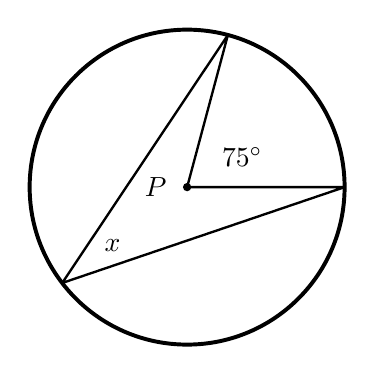
\begin{tikzpicture}[dot/.style={circle, fill=black, inner sep=0pt, outer sep=0pt, minimum size=3pt}, 
dim-label/.style={fill=white, rectangle, inner sep=2pt, outer sep=0pt}, 
nodot/.style={circle, fill=black, inner sep=0pt, outer sep=0pt, minimum size=0pt}, 
%remember picture, overlay
baseline = (current bounding box.west)
]  

% the origin 
\coordinate (p) at (0,0); 
% the circle and the nodot at the origin
\draw[line width=0.5mm] (p) node[circle, fill=black, inner sep=0pt, outer sep=0pt, minimum size=3pt] {} circle [radius=\rad2]; 

\node(p-label) at ($(p)+(180:0.2*\rad2)$) {$P$};

\node(p-angle) at ($(p)+(29:0.4*\rad2)$) {$75\degree$};

\node (a) at (0:\rad2) [nodot] {}; 

\node (b) at (75:\rad2) [nodot] {}; 


\node (c) at (217.5:\rad2) [nodot] {}; 

\node(x-label) at ($(c)+(37:0.4*\rad2)$) {$x$};


\draw[line width=0.3mm] (p)--(a)--(c) --(b) --(p) ; 


\end{tikzpicture} 
%2
\item \hspce 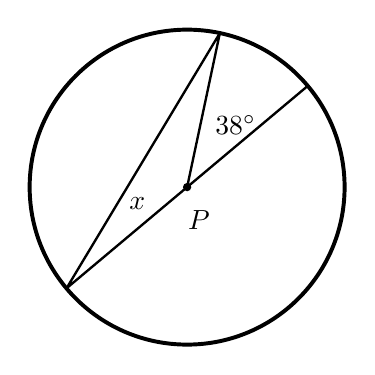
\begin{tikzpicture}[dot/.style={circle, fill=black, inner sep=0pt, outer sep=0pt, minimum size=3pt}, 
dim-label/.style={fill=white, rectangle, inner sep=2pt, outer sep=0pt}, 
nodot/.style={circle, fill=black, inner sep=0pt, outer sep=0pt, minimum size=0pt}, 
%remember picture, overlay
baseline = (current bounding box.west)
]  

\coordinate (p) at (0,0); 

\draw[line width=0.5mm] (p) node[circle, fill=black, inner sep=0pt, outer sep=0pt, minimum size=3pt] {} circle [radius=\rad2]; 

\node(p-label) at ($(p)+(290:0.22*\rad2)$) {$P$};

\node(p-angle) at ($(p)+(52:0.5*\rad2)$) {${38\degree}$};

\node (a) at (40:\rad2) [nodot] {}; 

\node (b) at (78:\rad2) [nodot] {}; 

\node (c) at (220:\rad2) [nodot] {};

\node(x-label) at ($(c)+(50:0.7*\rad2)$) {${x}$};
 
\draw[line width=0.3mm] (a)--(c)--(b)--(p) ; 

\end{tikzpicture} 
%3
\item \hspce 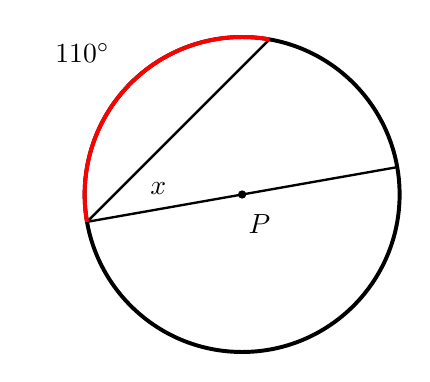
\begin{tikzpicture}[dot/.style={circle, fill=black, inner sep=0pt, outer sep=0pt, minimum size=3pt}, 
dim-label/.style={fill=white, rectangle, inner sep=2pt, outer sep=0pt}, 
nodot/.style={circle, fill=black, inner sep=0pt, outer sep=0pt, minimum size=0pt}, 
%remember picture, overlay
baseline = (current bounding box.west)
]  
\coordinate (p) at (0,0); 

\draw[line width=0.5mm] (p) node[circle, fill=black, inner sep=0pt, outer sep=0pt, minimum size=3pt] {} circle [radius=\rad2]; 

\node(p-label) at ($(p)+(-60:0.22*\rad2)$) {${P}$};

\node(angle) at ($(p)+(140:1.4*\rad2)$) {$ \  \ {110\degree}$};

\node (a) at (10:\rad2) [nodot] {}; 

\node (b) at (80:\rad2) [nodot] {}; 

\node (c) at (190:\rad2) [nodot] {};

\node(x-label) at ($(c)+(25:0.5*\rad2)$) {${x}$};
 
\draw[line width=0.3mm] (a)--(c) --(b); 

\draw[red, line width=0.5mm] (b)  arc (80:190:\rad2);

\end{tikzpicture} 
%4
\item \hspce 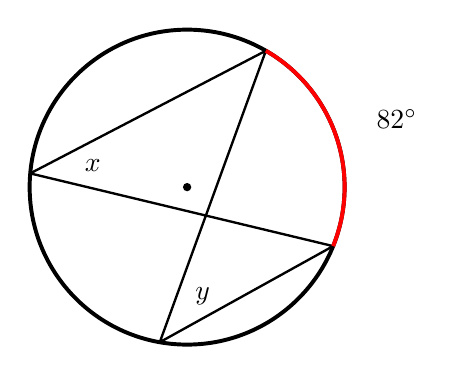
\begin{tikzpicture}[dot/.style={circle, fill=black, inner sep=0pt, outer sep=0pt, minimum size=3pt}, 
dim-label/.style={fill=white, rectangle, inner sep=2pt, outer sep=0pt}, 
nodot/.style={circle, fill=black, inner sep=0pt, outer sep=0pt, minimum size=0pt}, 
%remember picture, overlay
baseline = (current bounding box.west)
]  

\coordinate (p) at (0,0); 

\draw[line width=0.5mm] (p) node[circle, fill=black, inner sep=0pt, outer sep=0pt, minimum size=3pt] {} circle [radius=\rad2];
 
%\node(p-label) at ($(p)+(180:15pt)$) {$ \  \ {P}$};
\node(angle) at ($(p)+(18:1.4*\rad2)$) {${82\degree}$};

\node (a) at (60:\rad2) [nodot] {}; 

\node (b) at (175:\rad2) [nodot] {}; 

\node (c) at (260:\rad2) [nodot] {}; 

\node (d) at (-22:\rad2) [nodot] {};

\node(x-label) at ($(b)+(7:0.4*\rad2)$) {${x}$};

\node(y-label) at ($(c)+(47:0.4*\rad2)$) {${y}$};
 
\draw[line width=0.3mm] (a)--(b) --(d) --(c)--(a); 

\draw[red, line width=0.5mm] (d)  arc (-22:60:\rad2);

\end{tikzpicture} 
%5
\item \hspce 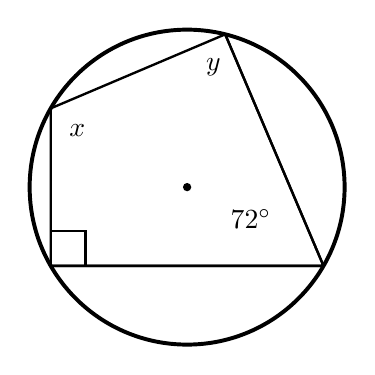
\begin{tikzpicture}[dot/.style={circle, fill=black, inner sep=0pt, outer sep=0pt, minimum size=3pt}, 
dim-label/.style={fill=white, rectangle, inner sep=2pt, outer sep=0pt}, 
nodot/.style={circle, fill=black, inner sep=0pt, outer sep=0pt, minimum size=0pt}, 
%remember picture, overlay
baseline = (current bounding box.west)
]  

\coordinate (p) at (0,0); 

\draw[line width=0.5mm] (p) node[circle, fill=black, inner sep=0pt, outer sep=0pt, minimum size=3pt] {} circle [radius=\rad2]; 

\node (a) at (76:\rad2) [nodot] {};

\node(y-label) at ($(a)+(250:0.22*\rad2)$) {${y}$};
  
\node (b) at (150:\rad2) [nodot] {};

\node(x-label) at ($(b)+(-40:0.22*\rad2)$) {${x}$};
 
\node (c) at (210:\rad2) [nodot] {}; 

\draw[line width=0.3mm] (c) rectangle ++(0.22*\rad2,0.22*\rad2) node[]{};

\node (d) at (-30:\rad2) [nodot] {}; 

\draw [line width=0.3mm](a) -- (d) -- (c) pic [draw,angle radius=0.3*\rad2] {angle = a--d--c}; 

\node(d-angle) at ($(d)+(150:0.6*\rad2)$) {$ \  \ {72\degree}$};

\draw[line width=0.3mm] (a)--(b) --(c) --(d) --(a) ; 

\end{tikzpicture} 
%6
\item \hspce 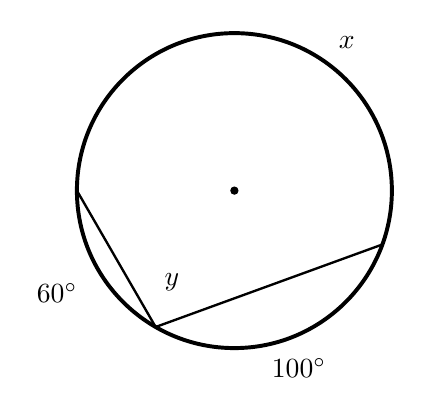
\begin{tikzpicture}[dot/.style={circle, fill=black, inner sep=0pt, outer sep=0pt, minimum size=3pt}, 
dim-label/.style={fill=white, rectangle, inner sep=2pt, outer sep=0pt}, 
nodot/.style={circle, fill=black, inner sep=0pt, outer sep=0pt, minimum size=0pt}, 
%remember picture, overlay
baseline = (current bounding box.west)
]  

\coordinate (p) at (0,0); 

\draw[line width=0.5mm] (p) node[circle, fill=black, inner sep=0pt, outer sep=0pt, minimum size=3pt] {} circle [radius=\rad2]; 

\node (a) at (180:\rad2) [nodot] {}; 

\node (b) at (240:\rad2) [nodot] {};

\node(y-label) at ($(b)+(70:0.3*\rad2)$) {${y}$};
 
\node (c) at (340:\rad2) [nodot] {}; 

\node(ab) at ($(p)+(210:1.3*\rad2)$) {${60\degree}$};

\node(x-label) at ($(c)+(100:1.3*\rad2)$) {$x$};
 
\node(bc) at ($(p)+(290:1.2*\rad2)$) {${100\degree}$};

\draw[line width=0.3mm] (a)--(b) --(c); 

\end{tikzpicture} 
%7
\item \hspce 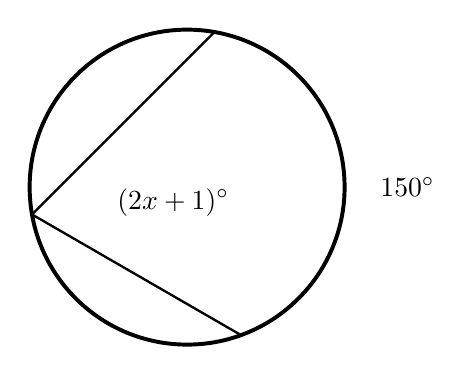
\begin{tikzpicture}[dot/.style={circle, fill=black, inner sep=0pt, outer sep=0pt, minimum size=3pt}, 
dim-label/.style={fill=white, rectangle, inner sep=2pt, outer sep=0pt}, 
nodot/.style={circle, fill=black, inner sep=0pt, outer sep=0pt, minimum size=0pt}, 
%remember picture, overlay
baseline = (current bounding box.west)
]  

\coordinate (p) at (0,0); 

\draw[line width=0.5mm] (p) node[circle, fill=black, inner sep=0pt, outer sep=0pt, minimum size=0pt] {} circle [radius=\rad2]; 

\node (a) at (80:\rad2) [nodot] {}; 

\node (b) at (190:\rad2) [nodot] {}; 

\node (c) at (-70:\rad2) [nodot] {}; 

\draw[line width=0.3mm] (a)--(b)--(c); 

\node(measure) at ($(b)+(5:0.9*\rad2)$) {${(2x+1)\degree}$};
 
\node(angle) at ($(p)+(0:1.4*\rad2)$) {${150\degree}$};
 
\end{tikzpicture} 
%8
\item \hspce 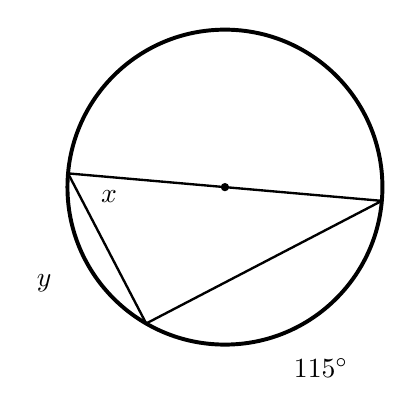
\begin{tikzpicture}[dot/.style={circle, fill=black, inner sep=0pt, outer sep=0pt, minimum size=3pt}, 
dim-label/.style={fill=white, rectangle, inner sep=2pt, outer sep=0pt}, 
nodot/.style={circle, fill=black, inner sep=0pt, outer sep=0pt, minimum size=0pt}, 
%remember picture, overlay
baseline = (current bounding box.west)
]  

\coordinate (p) at (0,0); 

\draw[line width=0.5mm] (p) node[circle, fill=black, inner sep=0pt, outer sep=0pt, minimum size=3pt] {} circle [radius=\rad2]; 

\node (a) at (-5:\rad2) [nodot] {}; 

\node (b) at (175:\rad2) [nodot] {}; 

\node (c) at (240:\rad2) [nodot] {}; 

\draw[line width=0.3mm] (a)--(b)--(c)--(a) ; 
 
\node(y-label) at ($(p)+(208:1.3*\rad2)$) {${y}$};
 
\node(x-label) at ($(b)+(-30:0.3*\rad2)$) {${x}$};
 
\node(115) at ($(p)+(298:1.3*\rad2)$) {${115\degree}$};
 
\end{tikzpicture} 
\end{multicols}
\end{enumerate}}     
\end{minipage}}
\end{center} 

B. $\Delta$GOA is inscribed in $\odot L$. If $m\angle{OGA}=75\degree$ and $m\arc{AG}=160\degree$, find: 
\begin{center}
\scalebox{1}{
\noindent\begin{minipage}{\textwidth}
 
{\begin{enumerate}[label = \arabic*. ]
\item $m\arc{OA}$ 
\item $m\arc{OG}$
\item $m\angle{GOA}$ \hspace*{3cm}\begin{tikzpicture}[dot/.style={circle, fill=black, inner sep=0pt, outer sep=0pt, minimum size=3pt}, 
dim-label/.style={fill=white, rectangle, inner sep=2pt, outer sep=0pt}, 
nodot/.style={circle, fill=black, inner sep=0pt, outer sep=0pt, minimum size=0pt}, 
remember picture, overlay
]  

\def\rad4{1.3cm}

\coordinate (l) at (0,0); 

\node(l-label) at ($(l)+(30:0.22*\rad4)$) {$L$};

\draw[line width=0.5mm] (l) node[circle, fill=black, inner sep=0pt, outer sep=0pt, minimum size=3pt] {} circle [radius=\rad4]; 

\node (a) at (15:\rad4) [nodot] {}; 

\node(a-label) at ($(a)+(15:0.22*\rad4)$) {$A$};
  
\node (o) at (165:\rad4) [nodot] {}; 

\node(o-label) at ($(o)+(165:0.22*\rad4)$) {$O$};
  
\node (g) at (215:\rad4) [nodot] {};

\node(g-label) at ($(g)+(215:0.22*\rad4)$) {$G$};
   
\node(75) at ($(g)+(53:0.4*\rad4)$) {$75\degree$};

\draw[line width=0.3mm] (a)--(o)--(g)--(a) ; 
 
\node(160) at ($(l)+(-45:1.3*\rad4)$) {$160\degree$};

\draw[red, line width=0.5mm] (a)  arc (15:-145:\rad4);

\end{tikzpicture} 
\item $m\angle{GAO}$  
\end{enumerate}}
\end{minipage}}
\end{center} 
\end{frame}

%\vspace*{-2.7in} %legalpaper
\vertadjust
\begin{frame} %3
\begin{center}
\textbf{Inscribed Angles and Intercepted Arcs}
\end{center}

\vspace*{1ex}
\begin{center}
\scalebox{1}{
\noindent\begin{minipage}{\textwidth}
{
\textbf{Inscribed angle: } an angle whose vertex lies on the circle and whose sides are chords of a circle

\vspce 

The measure of an inscribed angle is \textbf{half} the measure of its intercepted arc.

\vspce 

In a circle, if two inscribed angles intercept the same arc or congruent arcs, then the angles are congruent.

\vspce 

An angle inscribed in a semicircle is a right angle and therefore the measure is equal to $90\degree$.

\vspce 

If a quadrilateral is inscribed in a circle, then its opposite angles are supplementary.
}
\end{minipage}}
\end{center} 

 
\def\currentdir{/storage/emulated/0/Documents/documents/latex/1920/Grade-10/2nd/inscribed-angles-and-intercepted-arcs}


\textbf{Practice Exercises}

\vspce

A. Refer to $ \odot O$ to answer the following. 
\begin{center}
\scalebox{1}{
\noindent\begin{minipage}{\textwidth}
{\begin{enumerate}[label = \arabic*. ]
\item Name the angle that  intercept \arc{AP}. 
\item Name the angles that  intercept \arc{EV}. 
\item Name the arc that is  intercepted by $\angle{PAE}$. 
\item Name the arc that is intercepted \\ by $\angle{EVP}$. \hspace*{6cm}\vspace*{1ex}\begin{tikzpicture}[dot/.style={circle, fill=black, inner sep=0pt, outer sep=0pt, minimum size=3pt}, 
dim-label/.style={fill=white, rectangle, inner sep=2pt, outer sep=0pt}, 
nodot/.style={circle, fill=black, inner sep=0pt, outer sep=0pt, minimum size=0pt}, 
remember picture, overlay
]  

\def\rad1{1.2cm}

% the origin 
\coordinate (o) at (0,0); 
% the circle and the dot at the origin
\draw[line width=0.5mm] (o) node[circle, fill=black, inner sep=0pt, outer sep=0pt, minimum size=3pt] {} circle [radius=\rad1]; 

\node(o-label) at ($(o)+(200:0.22*\rad1)$) {$O$};

\node (e) at (90:\rad1) [nodot] {}; 
\node(e-label) at ($(e)+(90:0.22*\rad1)$) {$E$};

\node (v) at (20:\rad1) [nodot] {}; 
\node(v-label) at ($(v)+(20:0.22*\rad1)$) {$V$};

\node (a) at (270:\rad1) [nodot] {}; 
\node(a-label) at ($(a)+(270:0.22*\rad1)$) {$A$};

\node (p) at (180:\rad1) [nodot] {}; 
\node(p-label) at ($(p)+(180:0.22*\rad1)$) {$P$};

\node(r-label) at ($(o)+(115:0.4*\rad1)$) {$R$};

\draw[line width=0.3mm] (a)--(e); 
\draw[line width=0.3mm] (p)--(v); 
\draw[line width=0.3mm] (p)--(e)--(v) --(a) --(p) ; 

\node (Name) at (-45:1.3*\rad1) {$\odot{O}$}; 
\end{tikzpicture}

 
%\vspace*{-3ex}
\item If $m\angle{PEA}=48\degree $, then $m\arc{AP}=\blank$ \\ and $m\angle{AVP}=\blank$. 
\item $m\angle{EPA}=\blank$
\item $m\angle{EVP}+m\angle{PVA}=\blank$
\item  If $m\angle{VEP}=100\degree $, then $m\angle{PAV}=\blank$.
\end{enumerate}
}
\end{minipage}}
\end{center} 
%\begin{tikzpicture}[dot/.style={circle, fill=black, inner sep=0pt, outer sep=0pt, minimum size=3pt}, 
dim-label/.style={fill=white, rectangle, inner sep=2pt, outer sep=0pt}, 
nodot/.style={circle, fill=black, inner sep=0pt, outer sep=0pt, minimum size=0pt}, 
remember picture, overlay
]  

\def\rad1{1.2cm}

% the origin 
\coordinate (o) at (0,0); 
% the circle and the dot at the origin
\draw[line width=0.5mm] (o) node[circle, fill=black, inner sep=0pt, outer sep=0pt, minimum size=3pt] {} circle [radius=\rad1]; 

\node(o-label) at ($(o)+(200:0.22*\rad1)$) {$O$};

\node (e) at (90:\rad1) [nodot] {}; 
\node(e-label) at ($(e)+(90:0.22*\rad1)$) {$E$};

\node (v) at (20:\rad1) [nodot] {}; 
\node(v-label) at ($(v)+(20:0.22*\rad1)$) {$V$};

\node (a) at (270:\rad1) [nodot] {}; 
\node(a-label) at ($(a)+(270:0.22*\rad1)$) {$A$};

\node (p) at (180:\rad1) [nodot] {}; 
\node(p-label) at ($(p)+(180:0.22*\rad1)$) {$P$};

\node(r-label) at ($(o)+(115:0.4*\rad1)$) {$R$};

\draw[line width=0.3mm] (a)--(e); 
\draw[line width=0.3mm] (p)--(v); 
\draw[line width=0.3mm] (p)--(e)--(v) --(a) --(p) ; 

\node (Name) at (-45:1.3*\rad1) {$\odot{O}$}; 
\end{tikzpicture}




\def\currentdir{/storage/emulated/0/Documents/documents/latex/1920/Grade-10/2nd/inscribed-angles-and-intercepted-arcs}

\begin{center}
\scalebox{1}{
\noindent\begin{minipage}{\textwidth}
{
B. Given $\odot{S}, \overline{AR}\cong\overline{RO}\cong \overline{OS}\cong\overline{SA}, m\angle{AMR}=3x+20$ and $m\angle{OMR}=x+30$. Find each measure. 
\begin{enumerate}[label = \arabic*. ]
\item $x$
\item $m\angle{AMR}$
\item $m\angle{ORM}$
\item $m\arc{AM}$
\item $m\angle{RNO}$ \hspace*{4cm}
\begin{tikzpicture}[dot/.style={circle, fill=black, inner sep=0pt, outer sep=0pt, minimum size=3pt}, 
dim-label/.style={fill=white, rectangle, inner sep=2pt, outer sep=0pt}, 
nodot/.style={circle, fill=black, inner sep=0pt, outer sep=0pt, minimum size=0pt}, 
remember picture, overlay
]  

\def\rad3{1.5cm}

\coordinate (s) at (0,0);

\node (s-label) at ($(s)+ (-40:0.22*\rad3)$) {$S$}; 

\node (n-label) at ($(s)+ (80:0.65*\rad3)$) {$N$};

\draw[line width=0.5mm] (s) node[circle, fill=black, inner sep=0pt, outer sep=0pt, minimum size=3pt] {} circle [radius=\rad3]; 

\node (o) at (30:\rad3) [nodot] {};

\node (o-label) at ($(o)+ (30:0.22*\rad3  )$) {$O$};

\node (r) at (90:\rad3) [nodot] {}; 

\node (r-label) at ($(r)+ (90:0.22*\rad3  )$) {$R$};

\node (a) at (150:\rad3) [nodot] {};

\node (a-label) at ($(a)+ (150:0.22*\rad3 )$) {$A$};

\node (m) at (270:\rad3) [nodot] {};

\node (m-label) at ($(m)+ (270:0.22*\rad3  )$) {$ \  M$}; 

\draw[line width=0.3mm] (r)--(m)--(o)--(r)--(a)--(s)--(o)--(m)--(a)--(o) ; 
 
 
\node(name) at ($(s)+ (310:1.3*\rad3)$) {$\odot{S}$};
 
\end{tikzpicture} 
\item $m\angle{RAM}$
\item $m\arc{AR}$
\item $m\arc{OM}$
\item $m\angle{ROM}$
\item $m\angle{AMO}$
\end{enumerate}
}
\end{minipage}}
\end{center} 
%
\begin{tikzpicture}[dot/.style={circle, fill=black, inner sep=0pt, outer sep=0pt, minimum size=3pt}, 
dim-label/.style={fill=white, rectangle, inner sep=2pt, outer sep=0pt}, 
nodot/.style={circle, fill=black, inner sep=0pt, outer sep=0pt, minimum size=0pt}, 
remember picture, overlay
]  

\def\rad3{1.5cm}

\coordinate (s) at (0,0);

\node (s-label) at ($(s)+ (-40:0.22*\rad3)$) {$S$}; 

\node (n-label) at ($(s)+ (80:0.65*\rad3)$) {$N$};

\draw[line width=0.5mm] (s) node[circle, fill=black, inner sep=0pt, outer sep=0pt, minimum size=3pt] {} circle [radius=\rad3]; 

\node (o) at (30:\rad3) [nodot] {};

\node (o-label) at ($(o)+ (30:0.22*\rad3  )$) {$O$};

\node (r) at (90:\rad3) [nodot] {}; 

\node (r-label) at ($(r)+ (90:0.22*\rad3  )$) {$R$};

\node (a) at (150:\rad3) [nodot] {};

\node (a-label) at ($(a)+ (150:0.22*\rad3 )$) {$A$};

\node (m) at (270:\rad3) [nodot] {};

\node (m-label) at ($(m)+ (270:0.22*\rad3  )$) {$ \  M$}; 

\draw[line width=0.3mm] (r)--(m)--(o)--(r)--(a)--(s)--(o)--(m)--(a)--(o) ; 
 
 
\node(name) at ($(s)+ (310:1.3*\rad3)$) {$\odot{S}$};
 
\end{tikzpicture} 
%\def\currentdir{/storage/emulated/0/Documents/documents/latex/1920/Grade-10/2nd/inscribed-angles-and-intercepted-arcs}

\textbf{Problem Set}

\vspce

A. Use the
given figures to find the value of $x$ and $y$. 
\begin{center}
\scalebox{1}{
\noindent\begin{minipage}{\textwidth}
{\begin{enumerate}[label = \arabic*. ]
\begin{multicols}{2}
%1
\item \hspce \def\rad2{1.2cm}
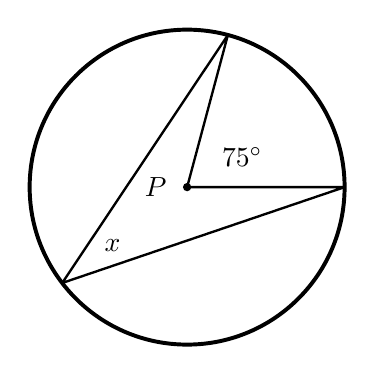
\begin{tikzpicture}[dot/.style={circle, fill=black, inner sep=0pt, outer sep=0pt, minimum size=3pt}, 
dim-label/.style={fill=white, rectangle, inner sep=2pt, outer sep=0pt}, 
nodot/.style={circle, fill=black, inner sep=0pt, outer sep=0pt, minimum size=0pt}, 
%remember picture, overlay
baseline = (current bounding box.west)
]  

% the origin 
\coordinate (p) at (0,0); 
% the circle and the nodot at the origin
\draw[line width=0.5mm] (p) node[circle, fill=black, inner sep=0pt, outer sep=0pt, minimum size=3pt] {} circle [radius=\rad2]; 

\node(p-label) at ($(p)+(180:0.2*\rad2)$) {$P$};

\node(p-angle) at ($(p)+(29:0.4*\rad2)$) {$75\degree$};

\node (a) at (0:\rad2) [nodot] {}; 

\node (b) at (75:\rad2) [nodot] {}; 


\node (c) at (217.5:\rad2) [nodot] {}; 

\node(x-label) at ($(c)+(37:0.4*\rad2)$) {$x$};


\draw[line width=0.3mm] (p)--(a)--(c) --(b) --(p) ; 


\end{tikzpicture} 
%2
\item \hspce 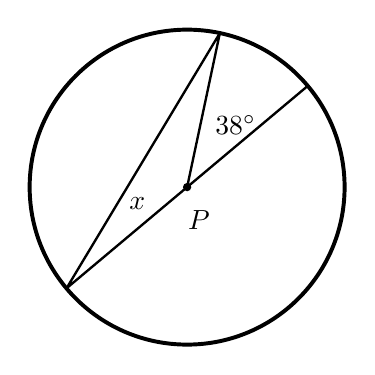
\begin{tikzpicture}[dot/.style={circle, fill=black, inner sep=0pt, outer sep=0pt, minimum size=3pt}, 
dim-label/.style={fill=white, rectangle, inner sep=2pt, outer sep=0pt}, 
nodot/.style={circle, fill=black, inner sep=0pt, outer sep=0pt, minimum size=0pt}, 
%remember picture, overlay
baseline = (current bounding box.west)
]  

\coordinate (p) at (0,0); 

\draw[line width=0.5mm] (p) node[circle, fill=black, inner sep=0pt, outer sep=0pt, minimum size=3pt] {} circle [radius=\rad2]; 

\node(p-label) at ($(p)+(290:0.22*\rad2)$) {$P$};

\node(p-angle) at ($(p)+(52:0.5*\rad2)$) {${38\degree}$};

\node (a) at (40:\rad2) [nodot] {}; 

\node (b) at (78:\rad2) [nodot] {}; 

\node (c) at (220:\rad2) [nodot] {};

\node(x-label) at ($(c)+(50:0.7*\rad2)$) {${x}$};
 
\draw[line width=0.3mm] (a)--(c)--(b)--(p) ; 

\end{tikzpicture} 
%3
\item \hspce 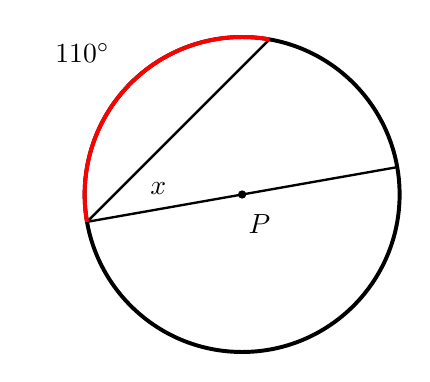
\begin{tikzpicture}[dot/.style={circle, fill=black, inner sep=0pt, outer sep=0pt, minimum size=3pt}, 
dim-label/.style={fill=white, rectangle, inner sep=2pt, outer sep=0pt}, 
nodot/.style={circle, fill=black, inner sep=0pt, outer sep=0pt, minimum size=0pt}, 
%remember picture, overlay
baseline = (current bounding box.west)
]  
\coordinate (p) at (0,0); 

\draw[line width=0.5mm] (p) node[circle, fill=black, inner sep=0pt, outer sep=0pt, minimum size=3pt] {} circle [radius=\rad2]; 

\node(p-label) at ($(p)+(-60:0.22*\rad2)$) {${P}$};

\node(angle) at ($(p)+(140:1.4*\rad2)$) {$ \  \ {110\degree}$};

\node (a) at (10:\rad2) [nodot] {}; 

\node (b) at (80:\rad2) [nodot] {}; 

\node (c) at (190:\rad2) [nodot] {};

\node(x-label) at ($(c)+(25:0.5*\rad2)$) {${x}$};
 
\draw[line width=0.3mm] (a)--(c) --(b); 

\draw[red, line width=0.5mm] (b)  arc (80:190:\rad2);

\end{tikzpicture} 
%4
\item \hspce 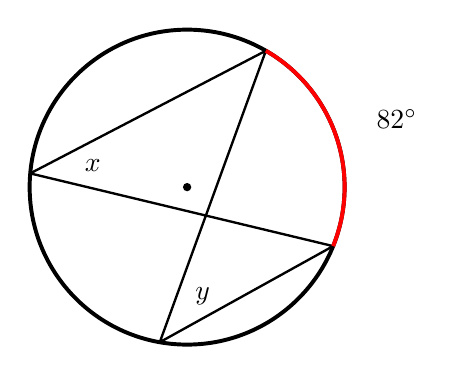
\begin{tikzpicture}[dot/.style={circle, fill=black, inner sep=0pt, outer sep=0pt, minimum size=3pt}, 
dim-label/.style={fill=white, rectangle, inner sep=2pt, outer sep=0pt}, 
nodot/.style={circle, fill=black, inner sep=0pt, outer sep=0pt, minimum size=0pt}, 
%remember picture, overlay
baseline = (current bounding box.west)
]  

\coordinate (p) at (0,0); 

\draw[line width=0.5mm] (p) node[circle, fill=black, inner sep=0pt, outer sep=0pt, minimum size=3pt] {} circle [radius=\rad2];
 
%\node(p-label) at ($(p)+(180:15pt)$) {$ \  \ {P}$};
\node(angle) at ($(p)+(18:1.4*\rad2)$) {${82\degree}$};

\node (a) at (60:\rad2) [nodot] {}; 

\node (b) at (175:\rad2) [nodot] {}; 

\node (c) at (260:\rad2) [nodot] {}; 

\node (d) at (-22:\rad2) [nodot] {};

\node(x-label) at ($(b)+(7:0.4*\rad2)$) {${x}$};

\node(y-label) at ($(c)+(47:0.4*\rad2)$) {${y}$};
 
\draw[line width=0.3mm] (a)--(b) --(d) --(c)--(a); 

\draw[red, line width=0.5mm] (d)  arc (-22:60:\rad2);

\end{tikzpicture} 
%5
\item \hspce 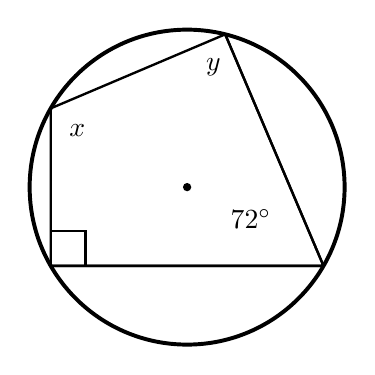
\begin{tikzpicture}[dot/.style={circle, fill=black, inner sep=0pt, outer sep=0pt, minimum size=3pt}, 
dim-label/.style={fill=white, rectangle, inner sep=2pt, outer sep=0pt}, 
nodot/.style={circle, fill=black, inner sep=0pt, outer sep=0pt, minimum size=0pt}, 
%remember picture, overlay
baseline = (current bounding box.west)
]  

\coordinate (p) at (0,0); 

\draw[line width=0.5mm] (p) node[circle, fill=black, inner sep=0pt, outer sep=0pt, minimum size=3pt] {} circle [radius=\rad2]; 

\node (a) at (76:\rad2) [nodot] {};

\node(y-label) at ($(a)+(250:0.22*\rad2)$) {${y}$};
  
\node (b) at (150:\rad2) [nodot] {};

\node(x-label) at ($(b)+(-40:0.22*\rad2)$) {${x}$};
 
\node (c) at (210:\rad2) [nodot] {}; 

\draw[line width=0.3mm] (c) rectangle ++(0.22*\rad2,0.22*\rad2) node[]{};

\node (d) at (-30:\rad2) [nodot] {}; 

\draw [line width=0.3mm](a) -- (d) -- (c) pic [draw,angle radius=0.3*\rad2] {angle = a--d--c}; 

\node(d-angle) at ($(d)+(150:0.6*\rad2)$) {$ \  \ {72\degree}$};

\draw[line width=0.3mm] (a)--(b) --(c) --(d) --(a) ; 

\end{tikzpicture} 
%6
\item \hspce 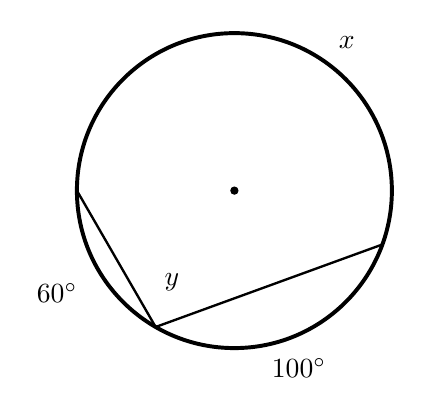
\begin{tikzpicture}[dot/.style={circle, fill=black, inner sep=0pt, outer sep=0pt, minimum size=3pt}, 
dim-label/.style={fill=white, rectangle, inner sep=2pt, outer sep=0pt}, 
nodot/.style={circle, fill=black, inner sep=0pt, outer sep=0pt, minimum size=0pt}, 
%remember picture, overlay
baseline = (current bounding box.west)
]  

\coordinate (p) at (0,0); 

\draw[line width=0.5mm] (p) node[circle, fill=black, inner sep=0pt, outer sep=0pt, minimum size=3pt] {} circle [radius=\rad2]; 

\node (a) at (180:\rad2) [nodot] {}; 

\node (b) at (240:\rad2) [nodot] {};

\node(y-label) at ($(b)+(70:0.3*\rad2)$) {${y}$};
 
\node (c) at (340:\rad2) [nodot] {}; 

\node(ab) at ($(p)+(210:1.3*\rad2)$) {${60\degree}$};

\node(x-label) at ($(c)+(100:1.3*\rad2)$) {$x$};
 
\node(bc) at ($(p)+(290:1.2*\rad2)$) {${100\degree}$};

\draw[line width=0.3mm] (a)--(b) --(c); 

\end{tikzpicture} 
%7
\item \hspce 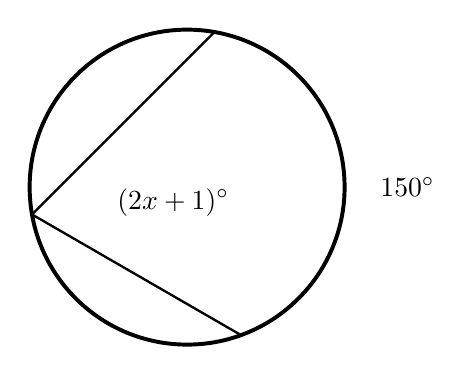
\begin{tikzpicture}[dot/.style={circle, fill=black, inner sep=0pt, outer sep=0pt, minimum size=3pt}, 
dim-label/.style={fill=white, rectangle, inner sep=2pt, outer sep=0pt}, 
nodot/.style={circle, fill=black, inner sep=0pt, outer sep=0pt, minimum size=0pt}, 
%remember picture, overlay
baseline = (current bounding box.west)
]  

\coordinate (p) at (0,0); 

\draw[line width=0.5mm] (p) node[circle, fill=black, inner sep=0pt, outer sep=0pt, minimum size=0pt] {} circle [radius=\rad2]; 

\node (a) at (80:\rad2) [nodot] {}; 

\node (b) at (190:\rad2) [nodot] {}; 

\node (c) at (-70:\rad2) [nodot] {}; 

\draw[line width=0.3mm] (a)--(b)--(c); 

\node(measure) at ($(b)+(5:0.9*\rad2)$) {${(2x+1)\degree}$};
 
\node(angle) at ($(p)+(0:1.4*\rad2)$) {${150\degree}$};
 
\end{tikzpicture} 
%8
\item \hspce 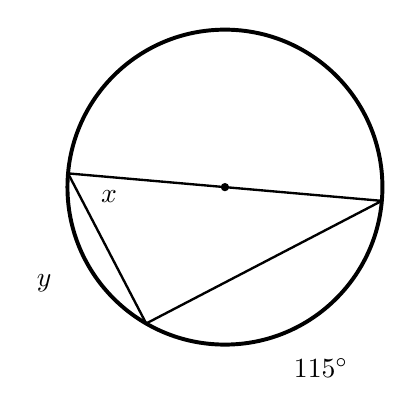
\begin{tikzpicture}[dot/.style={circle, fill=black, inner sep=0pt, outer sep=0pt, minimum size=3pt}, 
dim-label/.style={fill=white, rectangle, inner sep=2pt, outer sep=0pt}, 
nodot/.style={circle, fill=black, inner sep=0pt, outer sep=0pt, minimum size=0pt}, 
%remember picture, overlay
baseline = (current bounding box.west)
]  

\coordinate (p) at (0,0); 

\draw[line width=0.5mm] (p) node[circle, fill=black, inner sep=0pt, outer sep=0pt, minimum size=3pt] {} circle [radius=\rad2]; 

\node (a) at (-5:\rad2) [nodot] {}; 

\node (b) at (175:\rad2) [nodot] {}; 

\node (c) at (240:\rad2) [nodot] {}; 

\draw[line width=0.3mm] (a)--(b)--(c)--(a) ; 
 
\node(y-label) at ($(p)+(208:1.3*\rad2)$) {${y}$};
 
\node(x-label) at ($(b)+(-30:0.3*\rad2)$) {${x}$};
 
\node(115) at ($(p)+(298:1.3*\rad2)$) {${115\degree}$};
 
\end{tikzpicture} 
\end{multicols}
\end{enumerate}}     
\end{minipage}}
\end{center} 

B. $\Delta$GOA is inscribed in $\odot L$. If $m\angle{OGA}=75\degree$ and $m\arc{AG}=160\degree$, find: 
\begin{center}
\scalebox{1}{
\noindent\begin{minipage}{\textwidth}
 
{\begin{enumerate}[label = \arabic*. ]
\item $m\arc{OA}$ 
\item $m\arc{OG}$
\item $m\angle{GOA}$ \hspace*{3cm}\begin{tikzpicture}[dot/.style={circle, fill=black, inner sep=0pt, outer sep=0pt, minimum size=3pt}, 
dim-label/.style={fill=white, rectangle, inner sep=2pt, outer sep=0pt}, 
nodot/.style={circle, fill=black, inner sep=0pt, outer sep=0pt, minimum size=0pt}, 
remember picture, overlay
]  

\def\rad4{1.3cm}

\coordinate (l) at (0,0); 

\node(l-label) at ($(l)+(30:0.22*\rad4)$) {$L$};

\draw[line width=0.5mm] (l) node[circle, fill=black, inner sep=0pt, outer sep=0pt, minimum size=3pt] {} circle [radius=\rad4]; 

\node (a) at (15:\rad4) [nodot] {}; 

\node(a-label) at ($(a)+(15:0.22*\rad4)$) {$A$};
  
\node (o) at (165:\rad4) [nodot] {}; 

\node(o-label) at ($(o)+(165:0.22*\rad4)$) {$O$};
  
\node (g) at (215:\rad4) [nodot] {};

\node(g-label) at ($(g)+(215:0.22*\rad4)$) {$G$};
   
\node(75) at ($(g)+(53:0.4*\rad4)$) {$75\degree$};

\draw[line width=0.3mm] (a)--(o)--(g)--(a) ; 
 
\node(160) at ($(l)+(-45:1.3*\rad4)$) {$160\degree$};

\draw[red, line width=0.5mm] (a)  arc (15:-145:\rad4);

\end{tikzpicture} 
\item $m\angle{GAO}$  
\end{enumerate}}
\end{minipage}}
\end{center} 
\end{frame}

%\vspace*{-2.7in} %legalpaper
\vertadjust
\begin{frame} %4
%\begin{center}
\textbf{Inscribed Angles and Intercepted Arcs}
\end{center}

\vspace*{1ex}
\begin{center}
\scalebox{1}{
\noindent\begin{minipage}{\textwidth}
{
\textbf{Inscribed angle: } an angle whose vertex lies on the circle and whose sides are chords of a circle

\vspce 

The measure of an inscribed angle is \textbf{half} the measure of its intercepted arc.

\vspce 

In a circle, if two inscribed angles intercept the same arc or congruent arcs, then the angles are congruent.

\vspce 

An angle inscribed in a semicircle is a right angle and therefore the measure is equal to $90\degree$.

\vspce 

If a quadrilateral is inscribed in a circle, then its opposite angles are supplementary.
}
\end{minipage}}
\end{center} 

 
%\def\currentdir{/storage/emulated/0/Documents/documents/latex/1920/Grade-10/2nd/inscribed-angles-and-intercepted-arcs}


\textbf{Practice Exercises}

\vspce

A. Refer to $ \odot O$ to answer the following. 
\begin{center}
\scalebox{1}{
\noindent\begin{minipage}{\textwidth}
{\begin{enumerate}[label = \arabic*. ]
\item Name the angle that  intercept \arc{AP}. 
\item Name the angles that  intercept \arc{EV}. 
\item Name the arc that is  intercepted by $\angle{PAE}$. 
\item Name the arc that is intercepted \\ by $\angle{EVP}$. \hspace*{6cm}\vspace*{1ex}\begin{tikzpicture}[dot/.style={circle, fill=black, inner sep=0pt, outer sep=0pt, minimum size=3pt}, 
dim-label/.style={fill=white, rectangle, inner sep=2pt, outer sep=0pt}, 
nodot/.style={circle, fill=black, inner sep=0pt, outer sep=0pt, minimum size=0pt}, 
remember picture, overlay
]  

\def\rad1{1.2cm}

% the origin 
\coordinate (o) at (0,0); 
% the circle and the dot at the origin
\draw[line width=0.5mm] (o) node[circle, fill=black, inner sep=0pt, outer sep=0pt, minimum size=3pt] {} circle [radius=\rad1]; 

\node(o-label) at ($(o)+(200:0.22*\rad1)$) {$O$};

\node (e) at (90:\rad1) [nodot] {}; 
\node(e-label) at ($(e)+(90:0.22*\rad1)$) {$E$};

\node (v) at (20:\rad1) [nodot] {}; 
\node(v-label) at ($(v)+(20:0.22*\rad1)$) {$V$};

\node (a) at (270:\rad1) [nodot] {}; 
\node(a-label) at ($(a)+(270:0.22*\rad1)$) {$A$};

\node (p) at (180:\rad1) [nodot] {}; 
\node(p-label) at ($(p)+(180:0.22*\rad1)$) {$P$};

\node(r-label) at ($(o)+(115:0.4*\rad1)$) {$R$};

\draw[line width=0.3mm] (a)--(e); 
\draw[line width=0.3mm] (p)--(v); 
\draw[line width=0.3mm] (p)--(e)--(v) --(a) --(p) ; 

\node (Name) at (-45:1.3*\rad1) {$\odot{O}$}; 
\end{tikzpicture}

 
%\vspace*{-3ex}
\item If $m\angle{PEA}=48\degree $, then $m\arc{AP}=\blank$ \\ and $m\angle{AVP}=\blank$. 
\item $m\angle{EPA}=\blank$
\item $m\angle{EVP}+m\angle{PVA}=\blank$
\item  If $m\angle{VEP}=100\degree $, then $m\angle{PAV}=\blank$.
\end{enumerate}
}
\end{minipage}}
\end{center} 
%\begin{tikzpicture}[dot/.style={circle, fill=black, inner sep=0pt, outer sep=0pt, minimum size=3pt}, 
dim-label/.style={fill=white, rectangle, inner sep=2pt, outer sep=0pt}, 
nodot/.style={circle, fill=black, inner sep=0pt, outer sep=0pt, minimum size=0pt}, 
remember picture, overlay
]  

\def\rad1{1.2cm}

% the origin 
\coordinate (o) at (0,0); 
% the circle and the dot at the origin
\draw[line width=0.5mm] (o) node[circle, fill=black, inner sep=0pt, outer sep=0pt, minimum size=3pt] {} circle [radius=\rad1]; 

\node(o-label) at ($(o)+(200:0.22*\rad1)$) {$O$};

\node (e) at (90:\rad1) [nodot] {}; 
\node(e-label) at ($(e)+(90:0.22*\rad1)$) {$E$};

\node (v) at (20:\rad1) [nodot] {}; 
\node(v-label) at ($(v)+(20:0.22*\rad1)$) {$V$};

\node (a) at (270:\rad1) [nodot] {}; 
\node(a-label) at ($(a)+(270:0.22*\rad1)$) {$A$};

\node (p) at (180:\rad1) [nodot] {}; 
\node(p-label) at ($(p)+(180:0.22*\rad1)$) {$P$};

\node(r-label) at ($(o)+(115:0.4*\rad1)$) {$R$};

\draw[line width=0.3mm] (a)--(e); 
\draw[line width=0.3mm] (p)--(v); 
\draw[line width=0.3mm] (p)--(e)--(v) --(a) --(p) ; 

\node (Name) at (-45:1.3*\rad1) {$\odot{O}$}; 
\end{tikzpicture}




%\def\currentdir{/storage/emulated/0/Documents/documents/latex/1920/Grade-10/2nd/inscribed-angles-and-intercepted-arcs}

\begin{center}
\scalebox{1}{
\noindent\begin{minipage}{\textwidth}
{
B. Given $\odot{S}, \overline{AR}\cong\overline{RO}\cong \overline{OS}\cong\overline{SA}, m\angle{AMR}=3x+20$ and $m\angle{OMR}=x+30$. Find each measure. 
\begin{enumerate}[label = \arabic*. ]
\item $x$
\item $m\angle{AMR}$
\item $m\angle{ORM}$
\item $m\arc{AM}$
\item $m\angle{RNO}$ \hspace*{4cm}
\begin{tikzpicture}[dot/.style={circle, fill=black, inner sep=0pt, outer sep=0pt, minimum size=3pt}, 
dim-label/.style={fill=white, rectangle, inner sep=2pt, outer sep=0pt}, 
nodot/.style={circle, fill=black, inner sep=0pt, outer sep=0pt, minimum size=0pt}, 
remember picture, overlay
]  

\def\rad3{1.5cm}

\coordinate (s) at (0,0);

\node (s-label) at ($(s)+ (-40:0.22*\rad3)$) {$S$}; 

\node (n-label) at ($(s)+ (80:0.65*\rad3)$) {$N$};

\draw[line width=0.5mm] (s) node[circle, fill=black, inner sep=0pt, outer sep=0pt, minimum size=3pt] {} circle [radius=\rad3]; 

\node (o) at (30:\rad3) [nodot] {};

\node (o-label) at ($(o)+ (30:0.22*\rad3  )$) {$O$};

\node (r) at (90:\rad3) [nodot] {}; 

\node (r-label) at ($(r)+ (90:0.22*\rad3  )$) {$R$};

\node (a) at (150:\rad3) [nodot] {};

\node (a-label) at ($(a)+ (150:0.22*\rad3 )$) {$A$};

\node (m) at (270:\rad3) [nodot] {};

\node (m-label) at ($(m)+ (270:0.22*\rad3  )$) {$ \  M$}; 

\draw[line width=0.3mm] (r)--(m)--(o)--(r)--(a)--(s)--(o)--(m)--(a)--(o) ; 
 
 
\node(name) at ($(s)+ (310:1.3*\rad3)$) {$\odot{S}$};
 
\end{tikzpicture} 
\item $m\angle{RAM}$
\item $m\arc{AR}$
\item $m\arc{OM}$
\item $m\angle{ROM}$
\item $m\angle{AMO}$
\end{enumerate}
}
\end{minipage}}
\end{center} 
%
\begin{tikzpicture}[dot/.style={circle, fill=black, inner sep=0pt, outer sep=0pt, minimum size=3pt}, 
dim-label/.style={fill=white, rectangle, inner sep=2pt, outer sep=0pt}, 
nodot/.style={circle, fill=black, inner sep=0pt, outer sep=0pt, minimum size=0pt}, 
remember picture, overlay
]  

\def\rad3{1.5cm}

\coordinate (s) at (0,0);

\node (s-label) at ($(s)+ (-40:0.22*\rad3)$) {$S$}; 

\node (n-label) at ($(s)+ (80:0.65*\rad3)$) {$N$};

\draw[line width=0.5mm] (s) node[circle, fill=black, inner sep=0pt, outer sep=0pt, minimum size=3pt] {} circle [radius=\rad3]; 

\node (o) at (30:\rad3) [nodot] {};

\node (o-label) at ($(o)+ (30:0.22*\rad3  )$) {$O$};

\node (r) at (90:\rad3) [nodot] {}; 

\node (r-label) at ($(r)+ (90:0.22*\rad3  )$) {$R$};

\node (a) at (150:\rad3) [nodot] {};

\node (a-label) at ($(a)+ (150:0.22*\rad3 )$) {$A$};

\node (m) at (270:\rad3) [nodot] {};

\node (m-label) at ($(m)+ (270:0.22*\rad3  )$) {$ \  M$}; 

\draw[line width=0.3mm] (r)--(m)--(o)--(r)--(a)--(s)--(o)--(m)--(a)--(o) ; 
 
 
\node(name) at ($(s)+ (310:1.3*\rad3)$) {$\odot{S}$};
 
\end{tikzpicture} 
\def\currentdir{/storage/emulated/0/Documents/documents/latex/1920/Grade-10/2nd/inscribed-angles-and-intercepted-arcs}

\textbf{Problem Set}

\vspce

A. Use the
given figures to find the value of $x$ and $y$. 
\begin{center}
\scalebox{1}{
\noindent\begin{minipage}{\textwidth}
{\begin{enumerate}[label = \arabic*. ]
\begin{multicols}{2}
%1
\item \hspce \def\rad2{1.2cm}
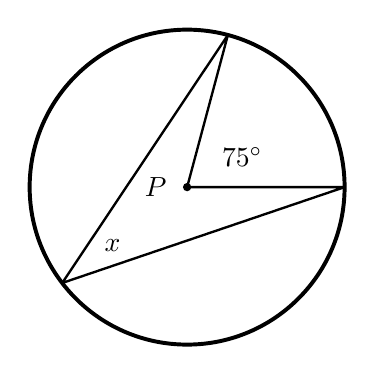
\begin{tikzpicture}[dot/.style={circle, fill=black, inner sep=0pt, outer sep=0pt, minimum size=3pt}, 
dim-label/.style={fill=white, rectangle, inner sep=2pt, outer sep=0pt}, 
nodot/.style={circle, fill=black, inner sep=0pt, outer sep=0pt, minimum size=0pt}, 
%remember picture, overlay
baseline = (current bounding box.west)
]  

% the origin 
\coordinate (p) at (0,0); 
% the circle and the nodot at the origin
\draw[line width=0.5mm] (p) node[circle, fill=black, inner sep=0pt, outer sep=0pt, minimum size=3pt] {} circle [radius=\rad2]; 

\node(p-label) at ($(p)+(180:0.2*\rad2)$) {$P$};

\node(p-angle) at ($(p)+(29:0.4*\rad2)$) {$75\degree$};

\node (a) at (0:\rad2) [nodot] {}; 

\node (b) at (75:\rad2) [nodot] {}; 


\node (c) at (217.5:\rad2) [nodot] {}; 

\node(x-label) at ($(c)+(37:0.4*\rad2)$) {$x$};


\draw[line width=0.3mm] (p)--(a)--(c) --(b) --(p) ; 


\end{tikzpicture} 
%2
\item \hspce 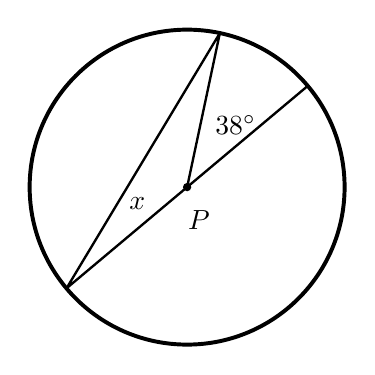
\begin{tikzpicture}[dot/.style={circle, fill=black, inner sep=0pt, outer sep=0pt, minimum size=3pt}, 
dim-label/.style={fill=white, rectangle, inner sep=2pt, outer sep=0pt}, 
nodot/.style={circle, fill=black, inner sep=0pt, outer sep=0pt, minimum size=0pt}, 
%remember picture, overlay
baseline = (current bounding box.west)
]  

\coordinate (p) at (0,0); 

\draw[line width=0.5mm] (p) node[circle, fill=black, inner sep=0pt, outer sep=0pt, minimum size=3pt] {} circle [radius=\rad2]; 

\node(p-label) at ($(p)+(290:0.22*\rad2)$) {$P$};

\node(p-angle) at ($(p)+(52:0.5*\rad2)$) {${38\degree}$};

\node (a) at (40:\rad2) [nodot] {}; 

\node (b) at (78:\rad2) [nodot] {}; 

\node (c) at (220:\rad2) [nodot] {};

\node(x-label) at ($(c)+(50:0.7*\rad2)$) {${x}$};
 
\draw[line width=0.3mm] (a)--(c)--(b)--(p) ; 

\end{tikzpicture} 
%3
\item \hspce 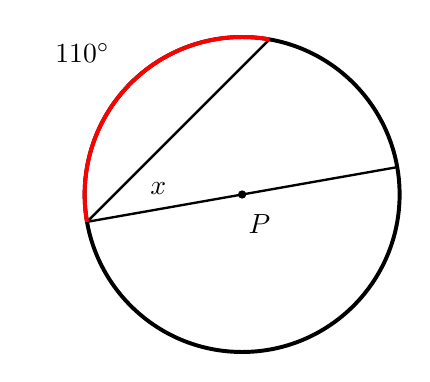
\begin{tikzpicture}[dot/.style={circle, fill=black, inner sep=0pt, outer sep=0pt, minimum size=3pt}, 
dim-label/.style={fill=white, rectangle, inner sep=2pt, outer sep=0pt}, 
nodot/.style={circle, fill=black, inner sep=0pt, outer sep=0pt, minimum size=0pt}, 
%remember picture, overlay
baseline = (current bounding box.west)
]  
\coordinate (p) at (0,0); 

\draw[line width=0.5mm] (p) node[circle, fill=black, inner sep=0pt, outer sep=0pt, minimum size=3pt] {} circle [radius=\rad2]; 

\node(p-label) at ($(p)+(-60:0.22*\rad2)$) {${P}$};

\node(angle) at ($(p)+(140:1.4*\rad2)$) {$ \  \ {110\degree}$};

\node (a) at (10:\rad2) [nodot] {}; 

\node (b) at (80:\rad2) [nodot] {}; 

\node (c) at (190:\rad2) [nodot] {};

\node(x-label) at ($(c)+(25:0.5*\rad2)$) {${x}$};
 
\draw[line width=0.3mm] (a)--(c) --(b); 

\draw[red, line width=0.5mm] (b)  arc (80:190:\rad2);

\end{tikzpicture} 
%4
\item \hspce 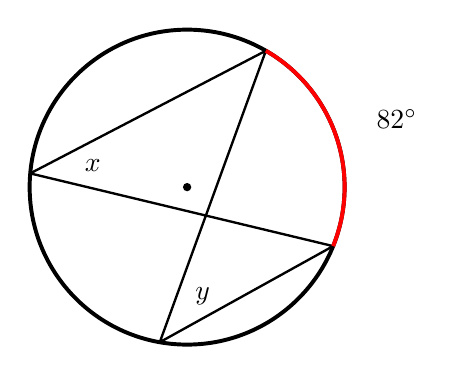
\begin{tikzpicture}[dot/.style={circle, fill=black, inner sep=0pt, outer sep=0pt, minimum size=3pt}, 
dim-label/.style={fill=white, rectangle, inner sep=2pt, outer sep=0pt}, 
nodot/.style={circle, fill=black, inner sep=0pt, outer sep=0pt, minimum size=0pt}, 
%remember picture, overlay
baseline = (current bounding box.west)
]  

\coordinate (p) at (0,0); 

\draw[line width=0.5mm] (p) node[circle, fill=black, inner sep=0pt, outer sep=0pt, minimum size=3pt] {} circle [radius=\rad2];
 
%\node(p-label) at ($(p)+(180:15pt)$) {$ \  \ {P}$};
\node(angle) at ($(p)+(18:1.4*\rad2)$) {${82\degree}$};

\node (a) at (60:\rad2) [nodot] {}; 

\node (b) at (175:\rad2) [nodot] {}; 

\node (c) at (260:\rad2) [nodot] {}; 

\node (d) at (-22:\rad2) [nodot] {};

\node(x-label) at ($(b)+(7:0.4*\rad2)$) {${x}$};

\node(y-label) at ($(c)+(47:0.4*\rad2)$) {${y}$};
 
\draw[line width=0.3mm] (a)--(b) --(d) --(c)--(a); 

\draw[red, line width=0.5mm] (d)  arc (-22:60:\rad2);

\end{tikzpicture} 
%5
\item \hspce 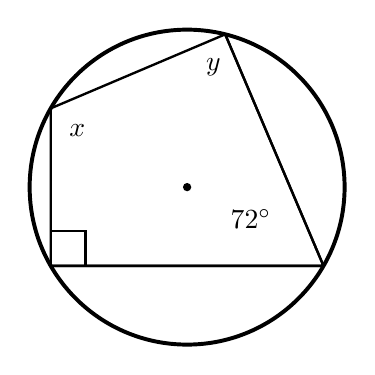
\begin{tikzpicture}[dot/.style={circle, fill=black, inner sep=0pt, outer sep=0pt, minimum size=3pt}, 
dim-label/.style={fill=white, rectangle, inner sep=2pt, outer sep=0pt}, 
nodot/.style={circle, fill=black, inner sep=0pt, outer sep=0pt, minimum size=0pt}, 
%remember picture, overlay
baseline = (current bounding box.west)
]  

\coordinate (p) at (0,0); 

\draw[line width=0.5mm] (p) node[circle, fill=black, inner sep=0pt, outer sep=0pt, minimum size=3pt] {} circle [radius=\rad2]; 

\node (a) at (76:\rad2) [nodot] {};

\node(y-label) at ($(a)+(250:0.22*\rad2)$) {${y}$};
  
\node (b) at (150:\rad2) [nodot] {};

\node(x-label) at ($(b)+(-40:0.22*\rad2)$) {${x}$};
 
\node (c) at (210:\rad2) [nodot] {}; 

\draw[line width=0.3mm] (c) rectangle ++(0.22*\rad2,0.22*\rad2) node[]{};

\node (d) at (-30:\rad2) [nodot] {}; 

\draw [line width=0.3mm](a) -- (d) -- (c) pic [draw,angle radius=0.3*\rad2] {angle = a--d--c}; 

\node(d-angle) at ($(d)+(150:0.6*\rad2)$) {$ \  \ {72\degree}$};

\draw[line width=0.3mm] (a)--(b) --(c) --(d) --(a) ; 

\end{tikzpicture} 
%6
\item \hspce 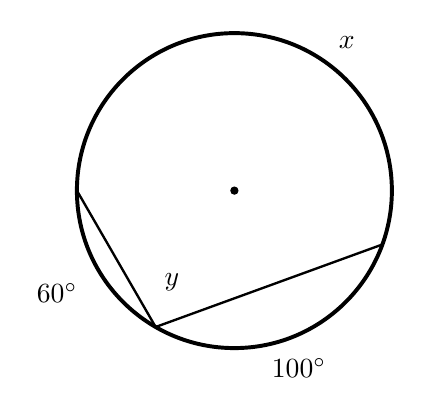
\begin{tikzpicture}[dot/.style={circle, fill=black, inner sep=0pt, outer sep=0pt, minimum size=3pt}, 
dim-label/.style={fill=white, rectangle, inner sep=2pt, outer sep=0pt}, 
nodot/.style={circle, fill=black, inner sep=0pt, outer sep=0pt, minimum size=0pt}, 
%remember picture, overlay
baseline = (current bounding box.west)
]  

\coordinate (p) at (0,0); 

\draw[line width=0.5mm] (p) node[circle, fill=black, inner sep=0pt, outer sep=0pt, minimum size=3pt] {} circle [radius=\rad2]; 

\node (a) at (180:\rad2) [nodot] {}; 

\node (b) at (240:\rad2) [nodot] {};

\node(y-label) at ($(b)+(70:0.3*\rad2)$) {${y}$};
 
\node (c) at (340:\rad2) [nodot] {}; 

\node(ab) at ($(p)+(210:1.3*\rad2)$) {${60\degree}$};

\node(x-label) at ($(c)+(100:1.3*\rad2)$) {$x$};
 
\node(bc) at ($(p)+(290:1.2*\rad2)$) {${100\degree}$};

\draw[line width=0.3mm] (a)--(b) --(c); 

\end{tikzpicture} 
%7
\item \hspce 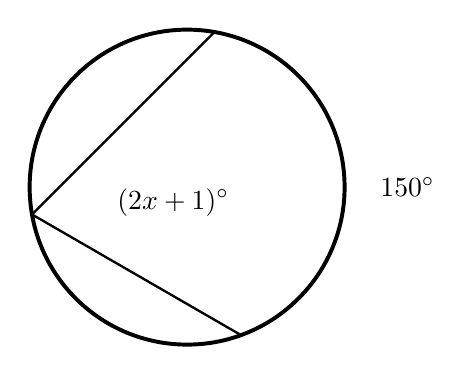
\begin{tikzpicture}[dot/.style={circle, fill=black, inner sep=0pt, outer sep=0pt, minimum size=3pt}, 
dim-label/.style={fill=white, rectangle, inner sep=2pt, outer sep=0pt}, 
nodot/.style={circle, fill=black, inner sep=0pt, outer sep=0pt, minimum size=0pt}, 
%remember picture, overlay
baseline = (current bounding box.west)
]  

\coordinate (p) at (0,0); 

\draw[line width=0.5mm] (p) node[circle, fill=black, inner sep=0pt, outer sep=0pt, minimum size=0pt] {} circle [radius=\rad2]; 

\node (a) at (80:\rad2) [nodot] {}; 

\node (b) at (190:\rad2) [nodot] {}; 

\node (c) at (-70:\rad2) [nodot] {}; 

\draw[line width=0.3mm] (a)--(b)--(c); 

\node(measure) at ($(b)+(5:0.9*\rad2)$) {${(2x+1)\degree}$};
 
\node(angle) at ($(p)+(0:1.4*\rad2)$) {${150\degree}$};
 
\end{tikzpicture} 
%8
\item \hspce \begin{tikzpicture}[dot/.style={circle, fill=black, inner sep=0pt, outer sep=0pt, minimum size=3pt}, 
dim-label/.style={fill=white, rectangle, inner sep=2pt, outer sep=0pt}, 
nodot/.style={circle, fill=black, inner sep=0pt, outer sep=0pt, minimum size=0pt}, 
%remember picture, overlay
baseline = (current bounding box.west)
]  

\coordinate (p) at (0,0); 

\draw[line width=0.5mm] (p) node[circle, fill=black, inner sep=0pt, outer sep=0pt, minimum size=3pt] {} circle [radius=\rad2]; 

\node (a) at (-5:\rad2) [nodot] {}; 

\node (b) at (175:\rad2) [nodot] {}; 

\node (c) at (240:\rad2) [nodot] {}; 

\draw[line width=0.3mm] (a)--(b)--(c)--(a) ; 
 
\node(y-label) at ($(p)+(208:1.3*\rad2)$) {${y}$};
 
\node(x-label) at ($(b)+(-30:0.3*\rad2)$) {${x}$};
 
\node(115) at ($(p)+(298:1.3*\rad2)$) {${115\degree}$};
 
\end{tikzpicture} 
\end{multicols}
\end{enumerate}}     
\end{minipage}}
\end{center} 

B. $\Delta$GOA is inscribed in $\odot L$. If $m\angle{OGA}=75\degree$ and $m\arc{AG}=160\degree$, find: 
\begin{center}
\scalebox{1}{
\noindent\begin{minipage}{\textwidth}
 
{\begin{enumerate}[label = \arabic*. ]
\item $m\arc{OA}$ 
\item $m\arc{OG}$
\item $m\angle{GOA}$ \hspace*{3cm}\begin{tikzpicture}[dot/.style={circle, fill=black, inner sep=0pt, outer sep=0pt, minimum size=3pt}, 
dim-label/.style={fill=white, rectangle, inner sep=2pt, outer sep=0pt}, 
nodot/.style={circle, fill=black, inner sep=0pt, outer sep=0pt, minimum size=0pt}, 
remember picture, overlay
]  

\def\rad4{1.3cm}

\coordinate (l) at (0,0); 

\node(l-label) at ($(l)+(30:0.22*\rad4)$) {$L$};

\draw[line width=0.5mm] (l) node[circle, fill=black, inner sep=0pt, outer sep=0pt, minimum size=3pt] {} circle [radius=\rad4]; 

\node (a) at (15:\rad4) [nodot] {}; 

\node(a-label) at ($(a)+(15:0.22*\rad4)$) {$A$};
  
\node (o) at (165:\rad4) [nodot] {}; 

\node(o-label) at ($(o)+(165:0.22*\rad4)$) {$O$};
  
\node (g) at (215:\rad4) [nodot] {};

\node(g-label) at ($(g)+(215:0.22*\rad4)$) {$G$};
   
\node(75) at ($(g)+(53:0.4*\rad4)$) {$75\degree$};

\draw[line width=0.3mm] (a)--(o)--(g)--(a) ; 
 
\node(160) at ($(l)+(-45:1.3*\rad4)$) {$160\degree$};

\draw[red, line width=0.5mm] (a)  arc (15:-145:\rad4);

\end{tikzpicture} 
\item $m\angle{GAO}$  
\end{enumerate}}
\end{minipage}}
\end{center} 
\end{frame}

\end{document}

